\chapter{The LHC and the CMS Detector} \label{chap-detector}

\section{The Large Hadron Collider} \label{sec-TheLargeHadronCollider}

The Large Hadron Collider (LHC) is currently the largest, and highest energy, particle accelerator ever created. Located, on average, one hundred metres under the Franco-Swiss border at Geneva, the LHC is installed in the 26.7 km tunnel that once contained the Large Electron-Positron Collider (LEP) which ran from 1989 until the end of 2000. The project was approved by the CERN council in December of 1994. Originally, the accelerator was designed as a two-stage project: constructed to run at a centre-of-mass energy of $\sqrt{s}=7$ TeV, and later an upgrade to $\sqrt{s}=14$ TeV. This was due to budget constraints which did not include contributions from non member states. 

After many setbacks, the first run began in 2010 and continued until the end of 2011 when the beam energy was then increased to $\sqrt{s}=8$ TeV for the whole of 2012 before shifting to Long Shutdown 1 (LS1) from 2013 to 2015. During LS1 the CERN accelerator complex, shown in Figure \ref{fig-CERNAcceleratorComplex}, was completely upgraded in order to run at a new unprecedented centre-of-mass energy of $\sqrt{s}=13$ TeV before ramping up to the original design energy of $\sqrt{s}=14$ TeV. 

\begin{figure}
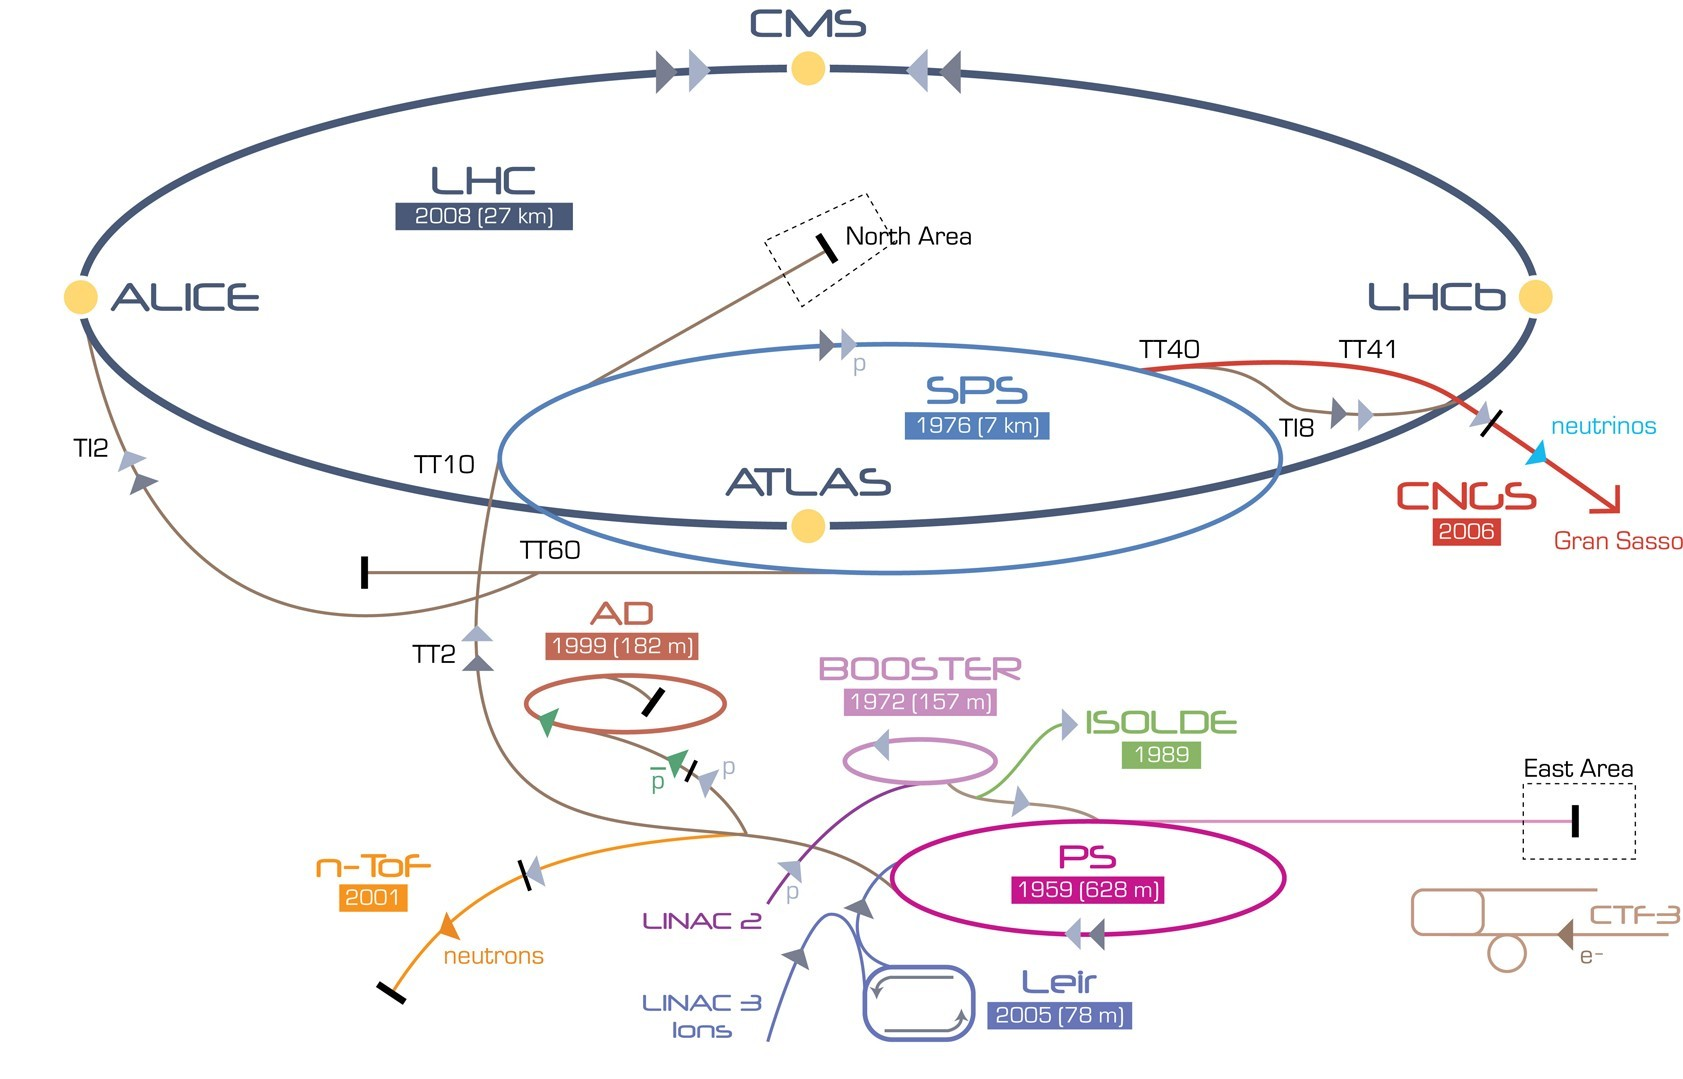
\includegraphics[width=\textwidth]{Figures/CERNAcceleratorComplex.jpg}
\caption{A full schematic of the full CERN accelerator complex.}
\label{fig-CERNAcceleratorComplex}
\end{figure}

\subsection{Pre-LHC accelerator complex}

The proton acceleration process begins by injecting Hydrogen ($H_2$) gas into a Duoplasmatron surrounded by an electric field, whereby the electrons become ionised through interactions with the free electrons from the cathode forming a plasma. This strips the electrons from the Hydroden leaving just the protons. The remaining protons are then linearly accelerated by the LINAC 2 accelerator, which uses radio frequency (RF) cavities to accelerate bunches of protons. By the end of this step the protons have reached an energy of up to 50 MeV and gained 5\% in mass. The next stage in the sequence sees the protons enter the Proton Synchroton Booster (PSB) which is composed of superimposed sychrotron rings which accelerate the received protons up to 1.4 GeV in 1.2 seconds before injection into the Proton Sychrotron (PS). The advantage of the Booster is that it allows the PS to accept over 100 times more protons by squeezing the proton bunches such that they have a much smaller cross-section. 

The PS is an essential component in the accelerator complex at CERN, where it accelerates either protons received from the PSB, or heavy ions from the Low Energy Ion Ring (LEIR). The apparatus first ran on the 24th of November 1959, and was, at that time, the worlds highest energy particle accelerator. Having a circumference of 628 metres, the PS comprises 277 conventional (room temperature) electromagnets, as well as 100 dipole magnets that serve to bend the beam around the ring. The PS accelerates protons, as well as other particles, up to 25 GeV in 3.2 s. The final stage of acceleration, before injection into the LHC, lies in the Super Proton Sychrotron (SPS). The SPS is the second largest of the CERN accelerators with a circumference of 7 kilometers, and provides beams for various experiments other than LHC: such as the NA61/SHINE and NA62 experiments, the COMPASS experiment, and the CNGS neutrino experiment. Protons are accelerated to 450 GeV  in 20 s within the SPS before injection into the LHC. Before the creation of LEP or the LHC the SPS was the primary collider at CERN, and in 1983 the collaboration won the Nobel prize for the discovery of the W and Z bosons in proton-antiproton collisions. The SPS comprises 1317 conventional electromagnets and 744 dipoles.

\subsection{Design of the LHC}

Two beams of protons are injected into the LHC and accelerated using RF cavities, one clockwise and the other counter-clockwise, taking roughly 20 minutes for each beam to reach the design energy of 7 TeV per beam. The two beams come into collision at four points around the $\sim27$ km ring where the collisions are recorded by the four detectors placed on the beam line. There are two all-purpose discovery detectors, namely CMS and ATLAS, studies of mesons by LHCb, and the ALICE experiment which has a primary focus on heavy ion studies. Because the tunnel in which the LHC is placed was designed for LEP it has an internal diameter of only 3.7 m, which is not large enough to install two separate beam pipes, and thus a design for a twin-bore magnet \cite{LHCStorageAccelerators} was created which would save space and cut costs substantially. Each beam is designed to hold 2808 bunches of protons with a bunch spacing of 50 ns. The protons are guided around the ring in a vacuum by superconducting electromagnets which are cooled to 1.9 K (-271.3$^\circ$) by using liquid helium. It consists of 1232 dipole magnets that are each 15 metres in length, and 392 quadrupole magnets that are 5-7 metres in length each which focus the beams. Before collisions can begin, a final shaping and cleaning of the beam takes place. Parameters for the LHC can be seen in Table \ref{tab-LHCparameters}.

\begin{table} 
\begin{center}
\begin{tabular}{|l|c|c|}
\hline
	\multicolumn{3}{|c|}{\textbf{LHC Parameters}} \\
\hline
	\textbf{Parameter} & \textbf{2012 Run} & \textbf{Design Value} \\
\hline	
	Beam Energy (TeV) & 4 & 7 \\
	Maximum number of bunches  & 1380 & 2808 \\
	Number of particles per bunch & $1.7\times 10^{11}$ & $1.15\times 10^{11}$ \\
	Bunch spacing (ns) & 50 & 25 \\
	Revolution frequency (kHz) & 11.245 & 11.245 \\
	Transverse beam size ($\mu$m) & 18.8 & 16.6 \\
	Peak luminosity (cm$^{-2}$s$^{-1}$) & $7.7\times 10^{33}$ & $10^{34}$ \\
	Stored beam energy (MJ) & 140 & 362 \\
	Normalised emittance at start of fill (mm mrad) & 2.5 & 3.75 \\
	$\beta^*$ in IP 1 and 5 (m) & 0.6 & 0.55 \\
\hline
\end{tabular}
\end{center}
\caption{LHC design parameters \cite{LHCDesignReport}.}
\label{tab-LHCparameters}
\end{table}


\subsection{Physics goals}

 There are many physics goals aimed to be achieved during the running of the LHC, but there are certain aims that are of a higher priority than others. One of the main focuses was the discovery of the Higgs boson and electroweak symmetry breaking, which was announced on the fourth of July 2012 \cite{CMSHiggs, ATLASHiggs}. This discovery was a triumph for the physics community in that it shed light on a fundamental building block of the universe which was theorised to exist some sixty years before its discovery. The theoretical physicists Peter Higgs and Fran\c{c}ois Englert subsequently won the Nobel prize for their work predicting the existence of a massive gauge boson as the mediator of the Higgs field in 1964. The Higgs a since been measured in various decay channels by both they ATLAS and CMS experiments with on-going studies aiming to measure properties of the boson, such as a the spin. Other physics goals include the search for supersymmetry, CP violation measurements, and studies of quark-gluon plasma using the ALICE experiment.  

\subsection{Luminosity at the LHC}

Due to the nature of individual detectors, not all require the same levels of delivered luminosity. For example, with CMS being an all-purpose discovery machine, the detector needs as much luminosity as possible, however an experiment like LHCb that measure mesons that are produced frequently and in a certain portion of the solid angle that the others use, less luminosity is required. The peak design luminosities for Run I and Run II are listed in Table \ref{tab-LHCparameters}. The instantaneous luminosity of a collider is calculated as

\begin{equation}
\mathcal{L}=f\frac{N_1N_2}{4\pi\sigma_x\sigma_y}
\end{equation}

where f is the collision frequency given by $f=u\times N_b$, the repetition frequency multiplied by the number of bunches in the beam, $N_{1,2}$ are the number of protons per bunch per beam, and $\sigma_{x,y}$ are the horizontal and vertical beam sizes at the interaction point (IP), respectively, and are defined as the product of the beams beta function and the proton beam emittance as shown in Equation \ref{eqn-beamsize}.

\begin{equation} \label{eqn-beamsize}
\sigma_{x,y}=\epsilon_{x,y}\beta_{x,y}
\end{equation}

The emittance of a beam describes the volume of the 6-dimensional phase space occupied by the proton bunch.

\subsection{Performance throughout run I}

Throughout Run I (2010 - 2013) the LHC operated with protons at beam energies of 3.5 and 4 TeV, where the beams consisted of single bunches and trains with different bunch spacing of 150 ns (2010), 75 ns (2011), and 50 ns (2011 and 2012). The performance of the LHC was much greater than initially expected at 50 ns, and culminated in the discovery of a $125$ $GeV/c^2$ Higgs boson in both the ATLAS \cite{ATLASHiggs} and CMS \cite{CMSHiggs} experiments. The use of 25 ns bunch spacing was only implemented in regards to electron-cloud scrubbing runs at the injection stage, and also for tests of future collisions with an upgraded LHC energy. One of the main focuses was to reduce the $\beta^*$ - the measure of how precisely the beam is focused at the interaction point. For ATLAS and CMS $\beta^*$ was lowered in steps from 3.5 mm in 2010 to 0.6 mm in 2012 by using tighter collimator settings. Other runs with mixed particle beams were also performed: such as proton-Pb, Pb-Pb, intermediate proton energy (1.38 TeV), and high beta.

For the 2012 run the default filling scheme introduced 1374 proton bunches per beam with 50 ns bunch spacing, giving ATLAS and CMS 1368 colliding bunches, 1262 in LHCb, and no colliding bunches in ALICE. The bunch intensity per beam peaked at $1.7 \times 10^{11}$ protons per bunch, which was then translated into a bunch intensity of $1.6 \times 10^{11}$ protons per bunch upon stabilisation of the beams. The transverse emittance remained constant throughout the year, despite moving to a different optical configuration with a lower transition energy. At the end of the runs the LHC had delivered an integrated luminosity of 23.3 fb$^{-1}$ to ATLAS and CMS, and over 2.1 fb$^{-1}$ to LHCb. The integrated and peak luminosity can be seen in Figure \ref{fig-LHClumi}, and the integrated luminosity recorded by CMS between 2011 ans 2013, and also compared to the total integrated luminosity delivered by the LHC, can be seen in Figure \ref{fig-CMSlumi}.

\newpage

\begin{figure} 
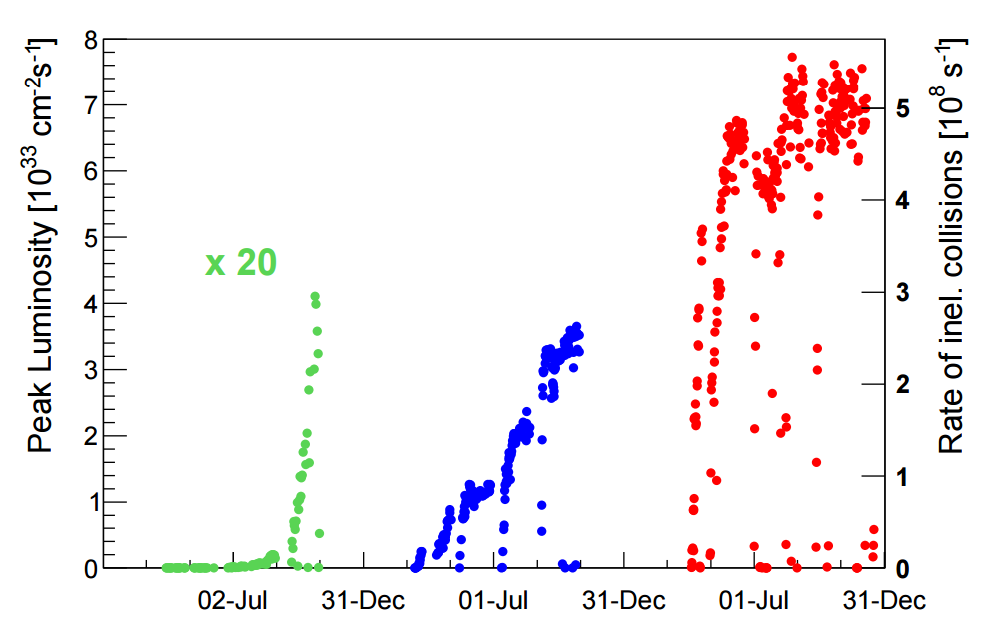
\includegraphics[width=0.5\textwidth]{Figures/LHClumi2.png}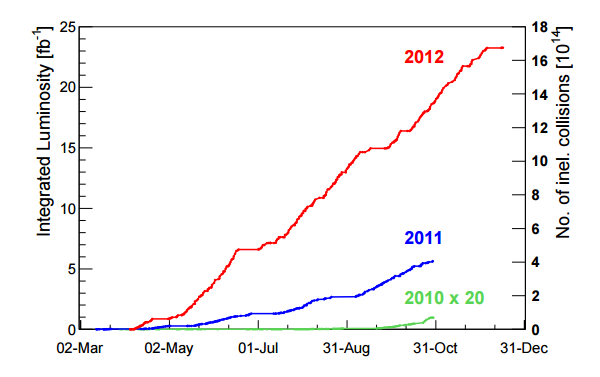
\includegraphics[width=0.5\textwidth]{Figures/LHClumi.png}
\caption{(Left) Peak and (right) integrated luminosity recorded by the LHC between 2010 and 2012 for proton operation. The 2010 luminosity values have been multiplied by a factor 20 \cite{LHClumi}.}
\label{fig-LHClumi}
\end{figure}

\begin{figure} 
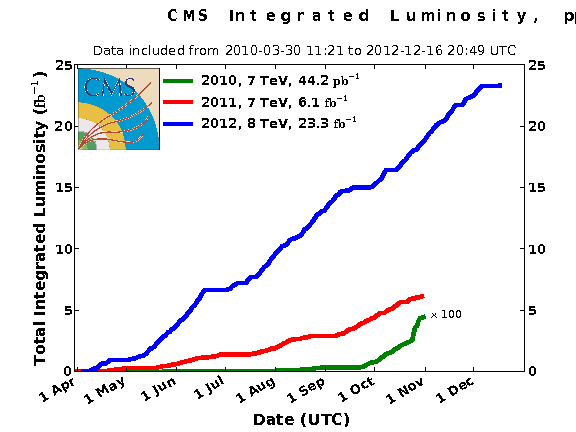
\includegraphics[width=0.5\textwidth]{Figures/IntLumi2.png}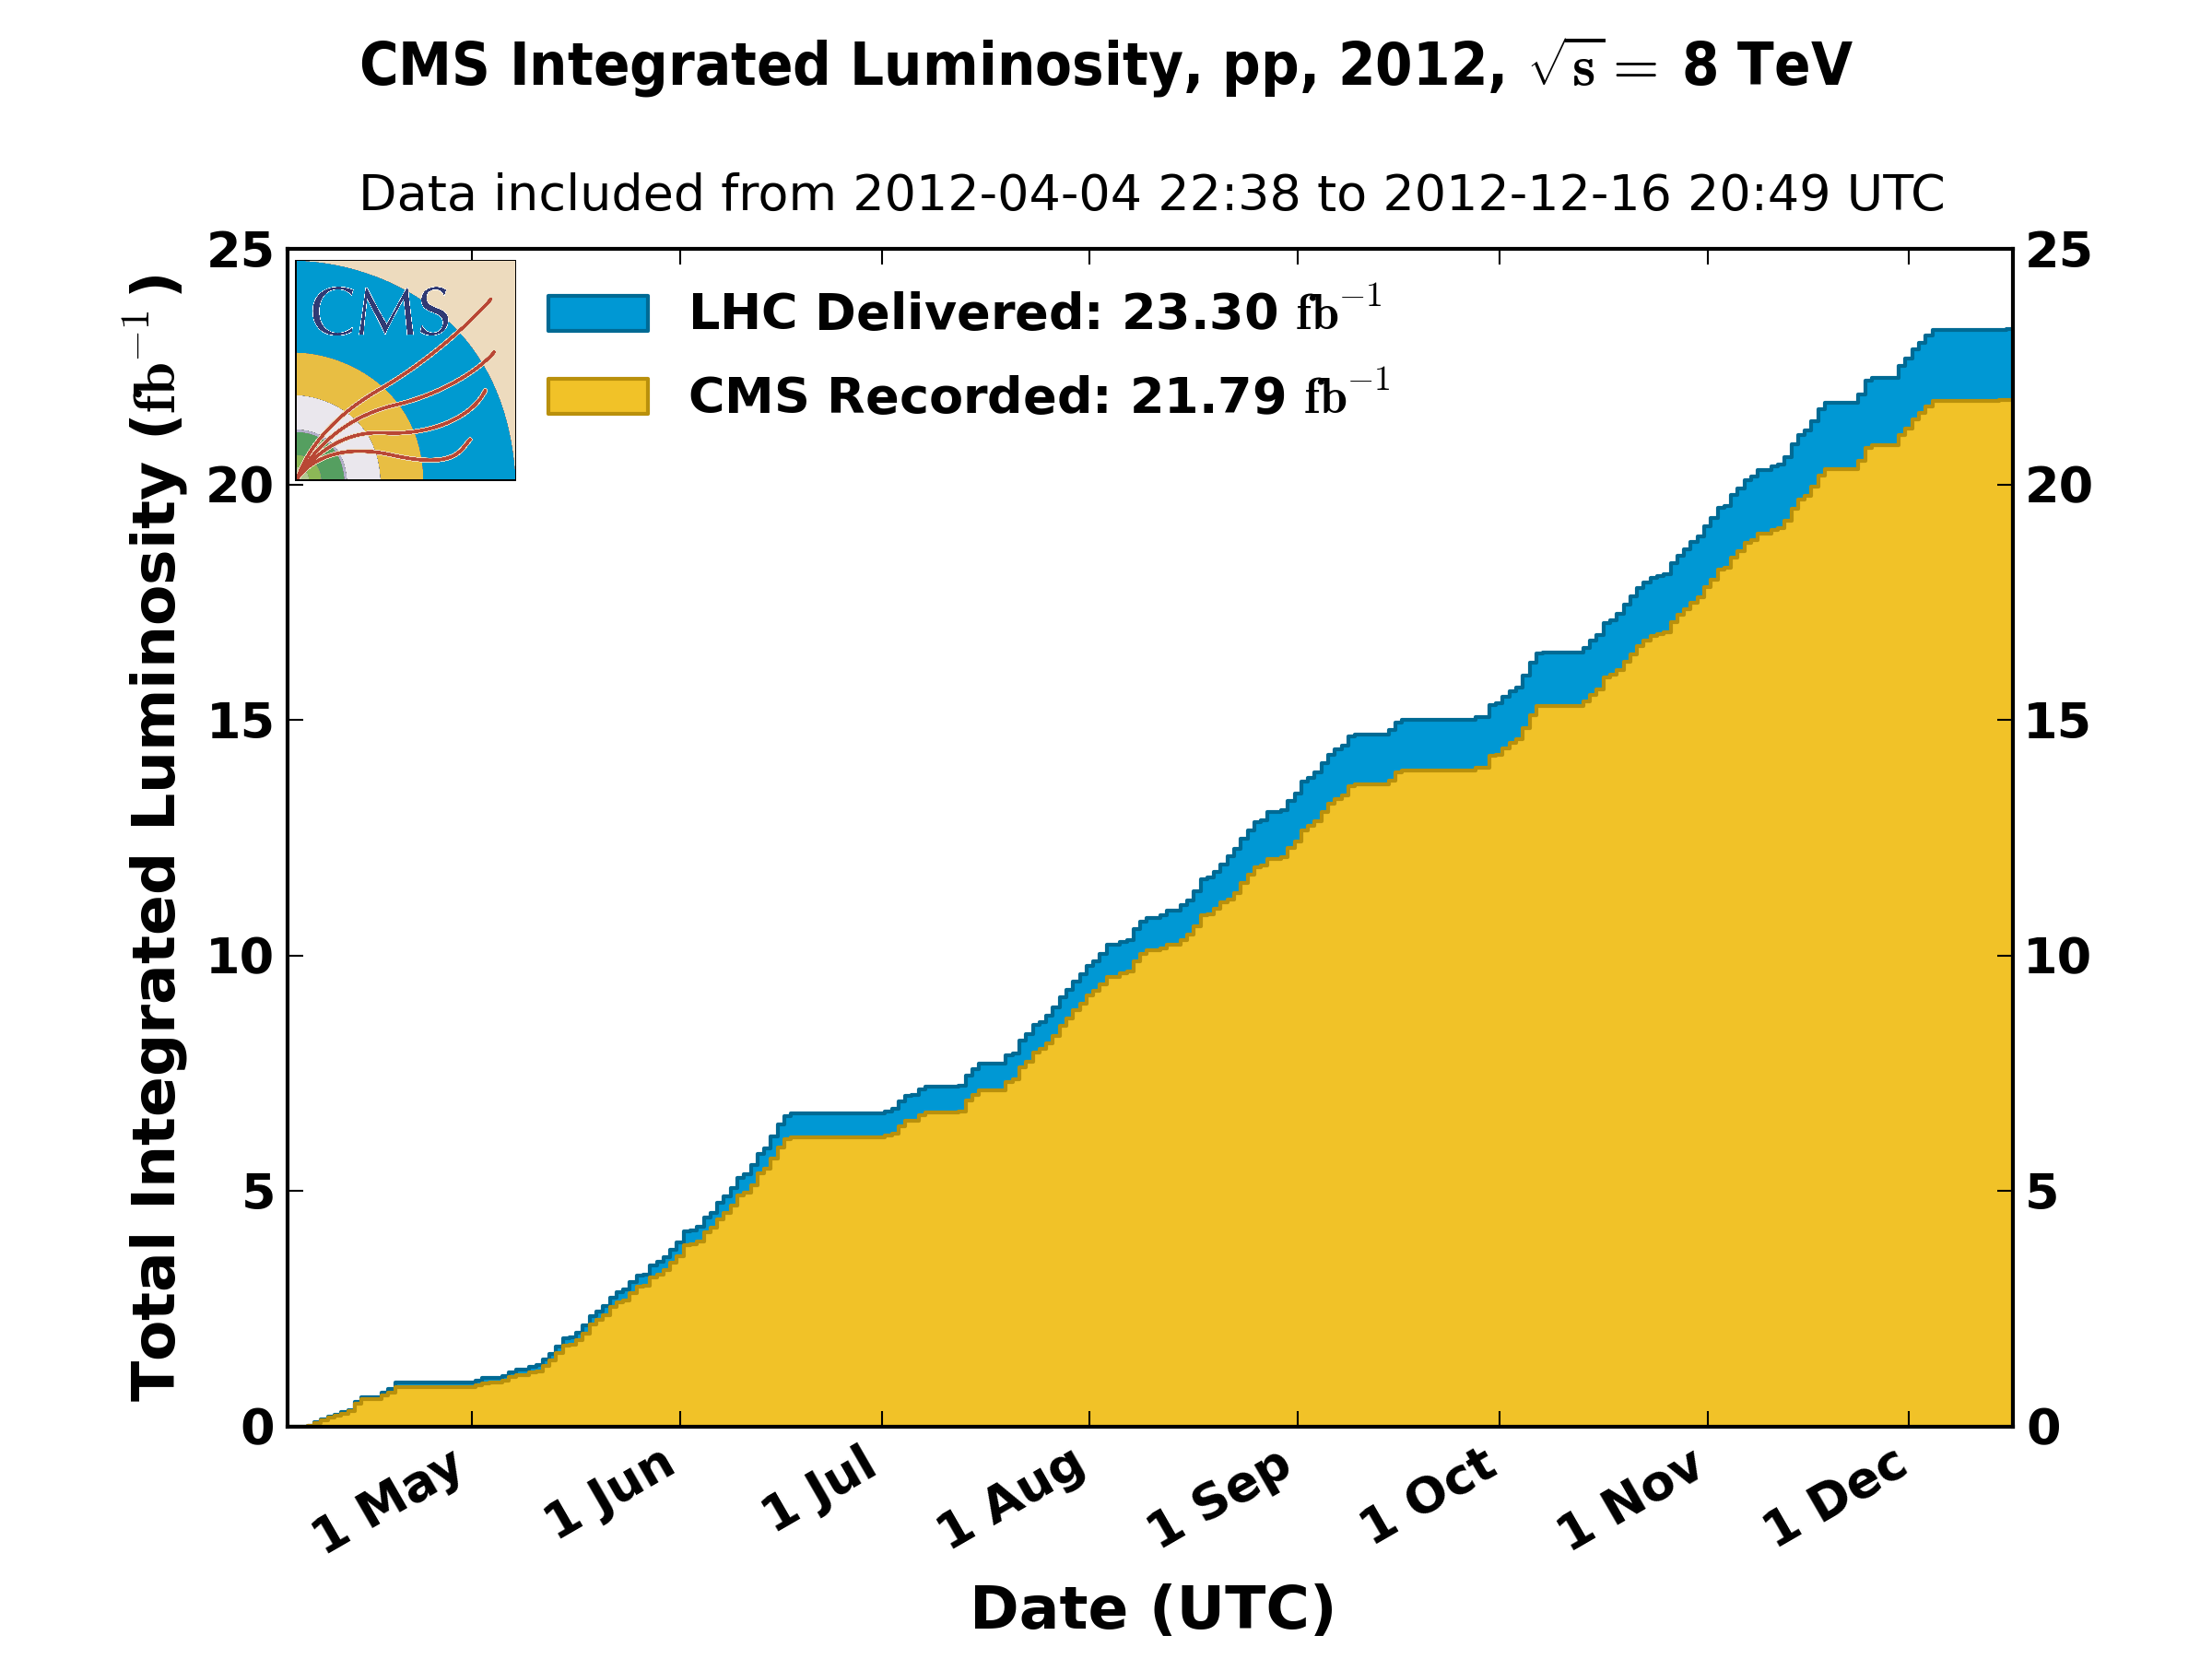
\includegraphics[width=0.5\textwidth]{Figures/CMSIntLumi.png}
\caption{Left: The accumulation of the integrated luminosity produced at the LHC vs time for runs in 2010, 2011, and 2012. The 2010 integrated luminosity is multiplied by 100 in order for it to be visible on the plot. Right: Total integrated luminosity vs time for the 2012 run in CMS and the LHC.}
\label{fig-CMSlumi}
\end{figure}

\newpage

\section{The CMS Detector} \label{sec-TheCMSDetector}

\begin{figure} [h!] 
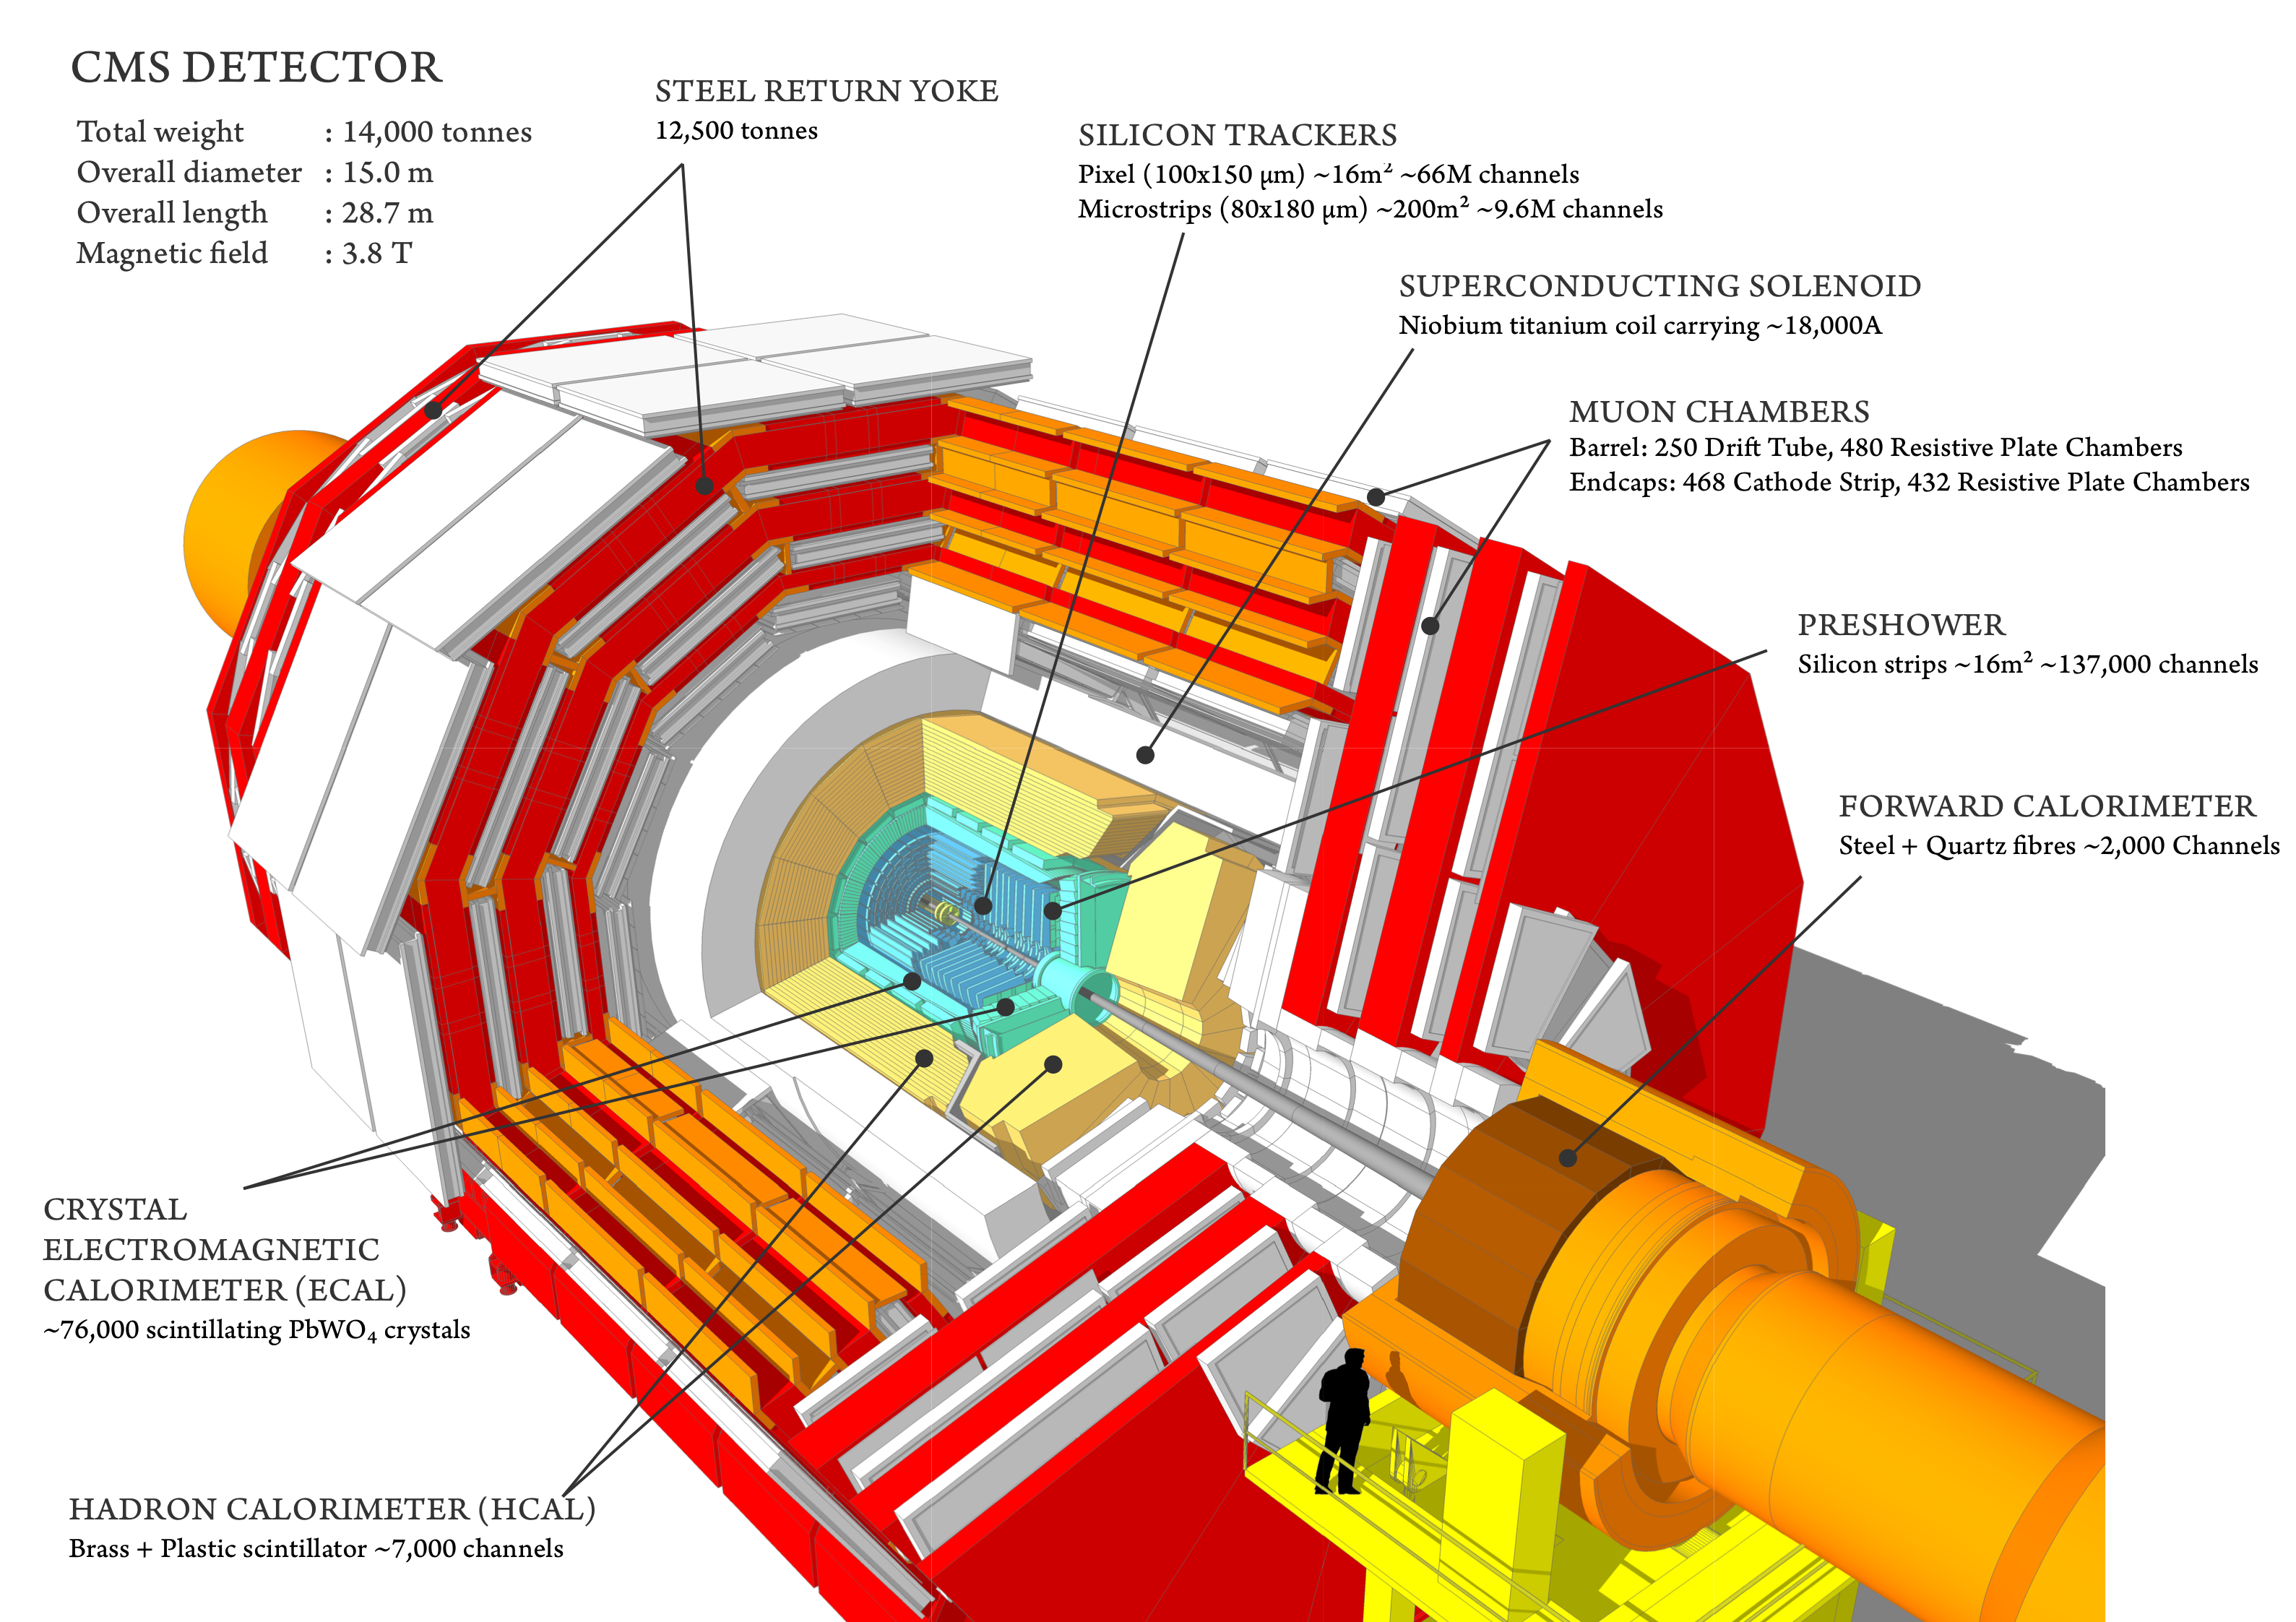
\includegraphics[width=\textwidth]{Figures/CMSDetector.png}
\caption{A cross-sectional view of the CMS detector.}
\label{fig-CMSDetector}
\end{figure}

The Compact Muon Solenoid (CMS) \cite{CMSexperiment} is one of the two all-purpose discovery machines located approximately 100 metres underground at point 5 (Cessy, France) on the LHC ring. Designed to cover the full solid angle, the hermetic detector is composed of multiple sub-detectors, described in detail in the following sections, designed to to perform precision particle detection and withstand extremely high doses of radiation. Unlike other detectors that lie on the LHC, besides the ATLAS experiment, ring CMS is designed with the purpose of precision measurements of Standard Model processes and the discovery of physics beyond that of the Standard Model. The primary physics motivation for the construction of such a detector was to elucidate the nature of electroweak symmetry breaking of which the Higgs field was theorised to be responsible, which was proved correct in 2012 with the discovery of the quanta that propagates the Higgs field - the Higgs boson. Many theories predict to observe new physics at the TeV scale, and so CMS was designed with the intention to be able to withstand high energy and fluence of particles. Discovering physics beyond the Standard Model would pave the way for a potential unified theory. The detector weighs around 14,000 tonnes and has an overall length of 28.7 metres and diameter of 15 metres. A sectional view of the CMS detector labeling each sub-detector within is shown in Figure \ref{fig-CMSDetector}. CMS uses a right-handed coordinate system whereby the x-axis points towards the center of the LHC ring, the y-axis lies perpendicular to the beam, and the z-axis follows the direction of the beam anti-clockwise. The azimuthal angle, $\phi$, is measured from the x-axis in the xy plane where the radial component in this plane is define by r, and the polar angle $\theta$ in the rz plane. The pseudorapitiy is thus defined as 

\begin{equation}
\eta = -\ln \left(\tan\left(\frac{\theta}{2}\right)\right)
\end{equation}

and the momentum transverse to the beam is defined as p$_T$, and calculated using the x- and y-components. The transverse energy is defined as E$_T = E\sin\theta$. 

\section{Inner Tracking System} \label{sec-InnerTrackingSystem}

The first sub-detector system located closest to the beam is the Inner Tracking System. The Inner Tracking System is composed of several modules that work in conjunction to provide precise and efficient measurements of the trajectories of charged particles resulting from the beam collisions, as well as a precision reconstruction of secondary vertices, whereby the product from the LHC beam collision decays. The tracker is completely hermetic around the interaction point (IP) of the beam-line, is 5.8 m in length, and has diameter of 2.5 m. In order to reconstruct particle tracks, measurements of the track's momentum must be made. To do this the tracker works in combination with the CMS Superconducting Solenoid (Section \ref{sec-SuperconductingSolenoid}) with a magnetic field at 4 T. 

Due to the high flux of the LHC at design luminosity the inner tracker will receive around 1000 particles per bunch crossing with around 20 primary vertices per collision, therefore the tracker was designed to operate with a high granularity and fast response time such that trajectories can be precisely identified and associated with the correct bunch crossing. Several challenges arise upon implementation of such technology: the requirement of high power density to the on-detector electronics means that sufficient cooling must be used throughout, which then conflicts with the ideology of keeping material to a minimum to prevent effects such as multiple scattering, bremsstrahlung, photon conversion, and nuclear scattering. Another challenge presents itself in the form of radiation damage to the tracking system due to the large flux of high energy particles over time. The requirements for a high granularity detector using minimum material that can run over a period of roughly 10 years whilst remaining radiation hard lead to a final design entirely based on silicon detector technology. 

Shown in Figure \ref{fig-Tracker}, the Inner Tracking System is composed of a pixel detector with a radii of between 4.4 cm and 10.2 cm, and a silicon strip tracker which in composed of 10 barrel detection layers reaching a radius of 1.1 m. In order to make tracking system hermetic the barrel detectors are surrounded by endcaps composed of 2 disks in the pixel detector and 3 plus 9 disks of silicon strip tracker, thus extending the acceptance, $A$, of the tracker up to a pseudorapidity of $|\eta| < 2.5$.  Each individual pixel station covers a region of $100\times150$ $\mu$m$^2$ in the $r-\phi$ and $z$ coordinate system, respectively. In total the pixel detector contains 66 million pixels, corresponding to an active area of 1 m$^2$.

\begin{figure} [h!] 
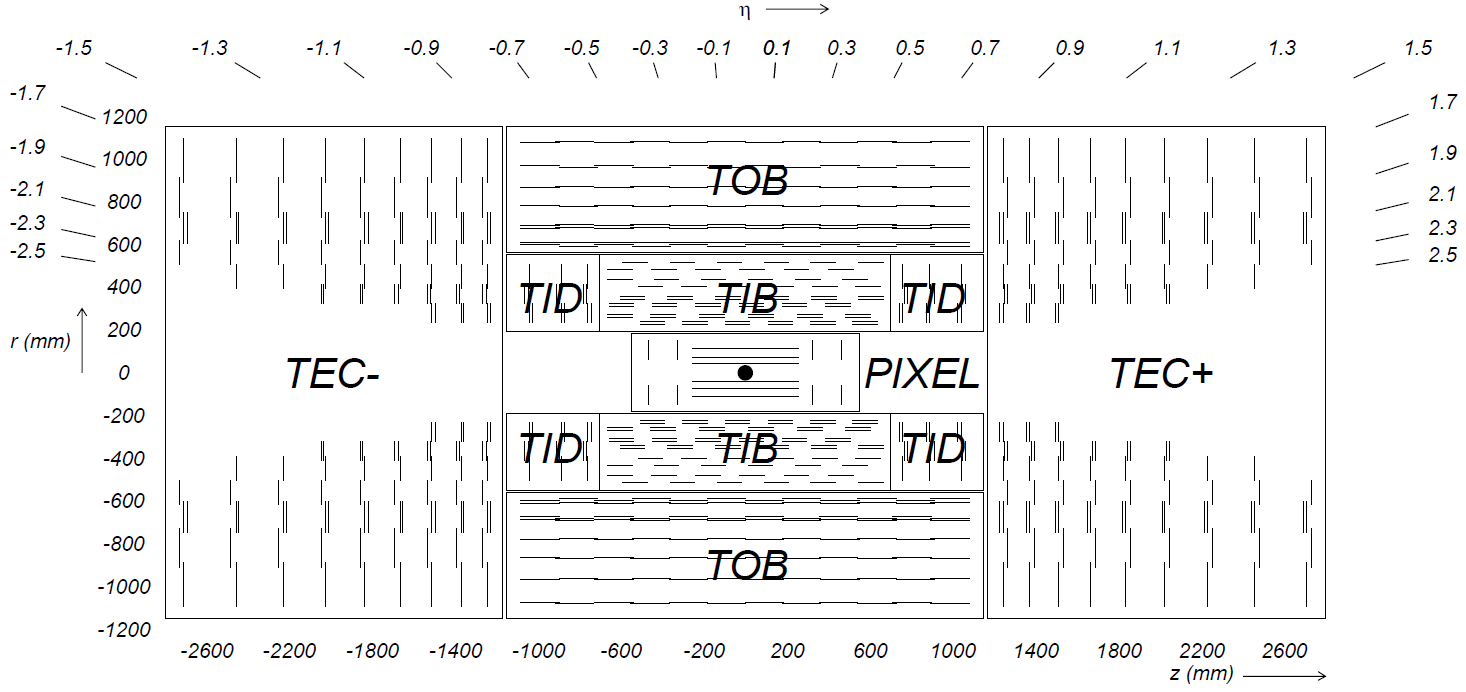
\includegraphics[width=\textwidth]{Figures/Tracker.png}
\caption{The sub-detectors of the CMS silicon tracker system: TOB=outer barrel, TIB=inner barrel, TID=inner disc, TEC=endcaps, PIXEL=pixeldetector. Each line represents a detector module. Double lines indicate back-to-back modules which deliver stereo hits. \cite{CMSexperiment}.}
\label{fig-Tracker}
\end{figure}

The sensor elements in the silicon strip tracker system are single sided p-on-n type silicon micro-strip sensors \cite{SiliconStripSensors1,SiliconStripSensors2}. The Tracker Inner Barrel (TIB) and Disks (TID), where the particle flux is smaller, extends to a radius of between 20 cm $< r <$ 55 cm, and has a typical cell size of 10 cm $\times 80 \mu$m$^2$, strip thickness of $320 \mu$m, and an occupancy of $\sim2-3\%$ per strip per bunch crossing. The outer layer of the silicon strip tracker ranges from 55 cm $< r <$ 110 cm and $\sim500 \mu$m thick, but with a cell size of 25 cm $\times$ 180 $\mu$m due to lower levels of radiation in the outer region. The TIB and TID are surrounded by the Tracker Outer Barrel (TOB) which has an outer radius of 116 cm and comprises 6 barrel layers of 500 $\mu$m thickness micro-strip sensors and strip patches of 183 $\mu$m on the first 4 layers and 122 $\mu$m on the 5th and 6th layers. Beyond the range of the TOB lies the Tracker EndCaps (TEC+ and TEC-, where the sign represents the location of the endcap along the z-axis) to provide complete coverage. The TECs cover the region 124 cm $<|z|<$ 282 cm and 22.5 cm $<|r|<$ 113.5 cm and is composed of 9 disks each consisting of 7 rings of silicon micro-strip detectors, 320 $\mu$m thick on the inner 4 rings, 500 $\mu$m thick on rings 5-7) with radial strips of 97 $\mu$m to 184 $\mu$m average pitch. Therefore, they provide up to 9 $\phi$ measurements per trajectory.

\subsection{Tracker performance in Run I} \label{subsec-TrackerPerformance}

Over the Run I period, from 2010 to 2013, the LHC delivered a luminosity of around 6 fb$^{-1}$ at 7 TeV and 23.3 fb$^{-1}$ at 8 TeV (Figure \ref{fig-LHClumi}), out of this approximately 93\% was recorded by CMS. The CMS tracker was responsible for roughly one third of the lost data due to the high voltage only being ramped up once stable beams are reached. By the end of Run I approximately 2.3\% of the tracker barrel and 7.2\% of the endcap modules were inactive associated with faulty wire-bonds or poor connections. During this period around 2.5\% of the strip detector became inactive because of short-circuits in the control rings and HV lines, or due to faulty optical communications. Maintenance and repairs began upon shut-down of the LHC, and CMS was able to salvage up to 1.5\% of the pixel barrel, up to 0.5\% of the pixel endcap modules, and up to 1\% of the strip detectors \cite{TrackerPerformance}.

In order to process the data prior to track reconstruction the hit efficiency must be measured, the points at which a charged particle traversed each layer of the inner tracker. After track reconstruction the efficiency is calculated as the fraction of particles that are expected to pass through the fiducial regions of the sensors in a layer of the detector in which matching hits are found. For the strip detectors a hit is considered to be a hit if the energy deposit is found in the module in which it was expected to be observed. For efficient reconstruction of tracks knowledge of the position of each module in three-dimensional space is required. Distortions and movements of the inner tracker modules were monitored using cosmic ray data and collision tracks by measuring the distance between expected and observed track trajectories. Distortions in tracking lead to biases in the reconstructed track curvature, and were studied using the reconstructed mass of $Z \to \mu\mu$ events as a function of the positive muon's azimuthal angle. The muon reconstruction efficiency can be seen in Figure \ref{fig-MuonReconstructionEfficiency}.

\begin{figure} 
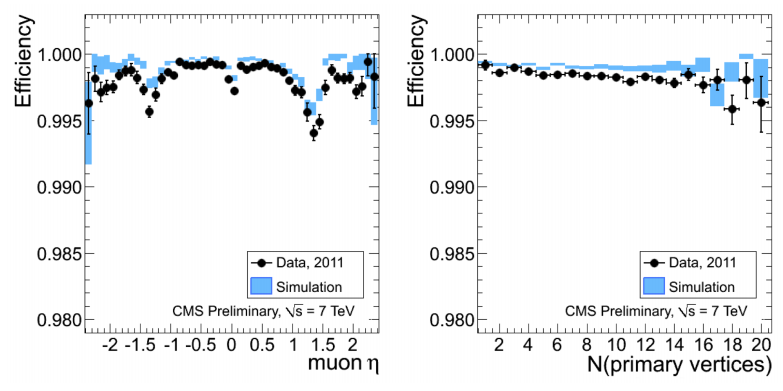
\includegraphics[width=\textwidth]{Figures/MuonReconstructionEfficiency.png}
\caption{Muon reconstruction efficiency in thee tracker as functions of pseudorapidity (left) and the number
of proton-proton interaction vertices (right) \cite{TrackingResults}.}
\label{fig-MuonReconstructionEfficiency}
\end{figure}

\begin{figure} 
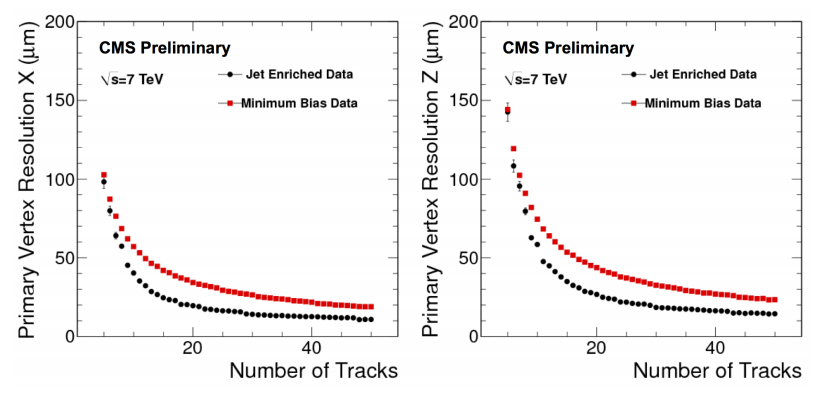
\includegraphics[width=\textwidth]{Figures/PVResolution.png}
\caption{Primary vertex resolution in the transverse plane (left) and along the beam-line (right) as functions
of the number of tracks attached to the vertex \cite{TrackingResults}.}
\label{fig-PVResolution}
\end{figure}

The CMS tracking software relies on an iterative procedure to measure hits in a high particle occupancy environment. Earlier steps of the tracking process search for tracks with higher p$_T$ due to the more obvious nature of the tracks, which include a smaller impact parameter, and greater number of measured hits in each layer of the tracker. By selecting more obvious processes first, the reconstruction becomes easier as it has fewer events to deal with. Track reconstruction efficiency is measured by using the tag-and-probe method in $Z \to \mu\mu$ events \cite{TrackingResults}. The tracking efficiency is then defined as the number of probes observed to have matching tracks within the tracker and is a function of the number of primary vertices and the pseudorapidity of the tracks and can be seen in Figure \ref{fig-PVResolution}. LHC proton-proton events are reconstructed by firstly identifying the tracks, then grouping in accordance with their primary vertex, and finally fitting to the position of each vertex.  

One of the long term damaging effects of high luminosity collisions is radiation damage. Radiation damage in the silicon was monitored throughout Run I and tested by performing special runs where the bias voltage was increased in steps from 0 to the operational voltages. Results showed that the hit efficiency decreased with irradiation at first, then increased with changes in the effective doping \cite{Doping}. Due to collisions not being completely aligned at the centre of the detector, even irradiation of the modules is seen in the azimuthal direction.

Overall, the CMS tracker has performed exceptionally throughout the Run I three-year period with regards to detector reliability and tracking. The tracker was able to overcome a major problem of high pile-up and reconstruct tracks with excellent efficiency. Less than 3\% of the tracker became inactive throughout the entire run, and less than 5\% of the delivered luminosity was lost through the tracker.    
 
\section{Electromagnetic Calorimeter} \label{sec-ElectromagneticCalorimeter}

\subsection{Overview} \label{subsec-ECALOverview}

Directly after the Inner Tracking System, the second stage of particle identification and reconstruction comes in the form of the Electromagnetic Calorimeter (ECAL). The ECAL serves to stop electromagnetic particles, namely electrons and photons, and measure the energy deposited in the detector. These particles are identified and reconstructed using signatures such as charge, shower shape, and isolation. When an electron passes through the ECAL it showers via bremsstrahlung, positron pair annihilation, and photon conversion. Radiation losses due to bremsstrahlung scale with mass as m$^{-4}$ (m$^{-6}$) when a charged particle travels perpendicular (parallel) to an electric field, and thus heavier electromagnetic particles are less likely to produce a shower. It is possible to differentiate between electrons and positrons by the curvature produced from the Superconducting Solenoid. Photons are neutrally charged and thus do not bend via the magnet, however they produce and electron-positron pair which then showers in the detector in the same manner as an incident electron, which can then be measured. The photon shower shape, known as $\sigma_{i\eta i\eta}$, is a prominent variable in this analysis and will be described in detail in Section \ref{chap-EventSelection}.  

A key component that drove the design of the ECAL is the decay channel $H \to \gamma\gamma$. At the time of design, the Higgs had not been discovered and thus the mass was not known, however it was known that the aforementioned decay mode was sensitive to a low mass Higgs, $m_H<150$ GeV. Although the branching ratio of the decay is small ($\simeq0.002$), the signature is clean and is a narrow resonance of two high E$_T$ photons over a non resonant background \cite{HiggsProposal}. In order to discover the Higgs the detector needed to have a powerful invariant mass resolution and background rejection, translating into a need for extremely efficient photon and electron identification, along with a high position and energy resolution. 

\subsection{Composition of the ECAL} \label{subsec-ECALComposition}

The CMS ECAL is a is a hermetic, homogeneous fine-grained lead tungstate (PbWO$_4$) crystal calorimeter \cite{ECAL}, shown in Figure \ref{fig-ECAL}. The PbWO$_4$ crystals are extremely dense  ($\delta=8.28$ g/cm$^3$), thus providing excellent performance and compactness, and thus fit within the Superconducting Solenoid magnet volume. The crystals have an extremely small radiation length, $X_0=0.85$ cm, and small Moli\`{e}re radius, $R_M=2.19$ cm. The decision to use a homogeneous medium was chosen because of the ability to obtain a greater energy resolution by minimizing fluctuations \cite{ECAL}. 

\begin{figure} [h!] 
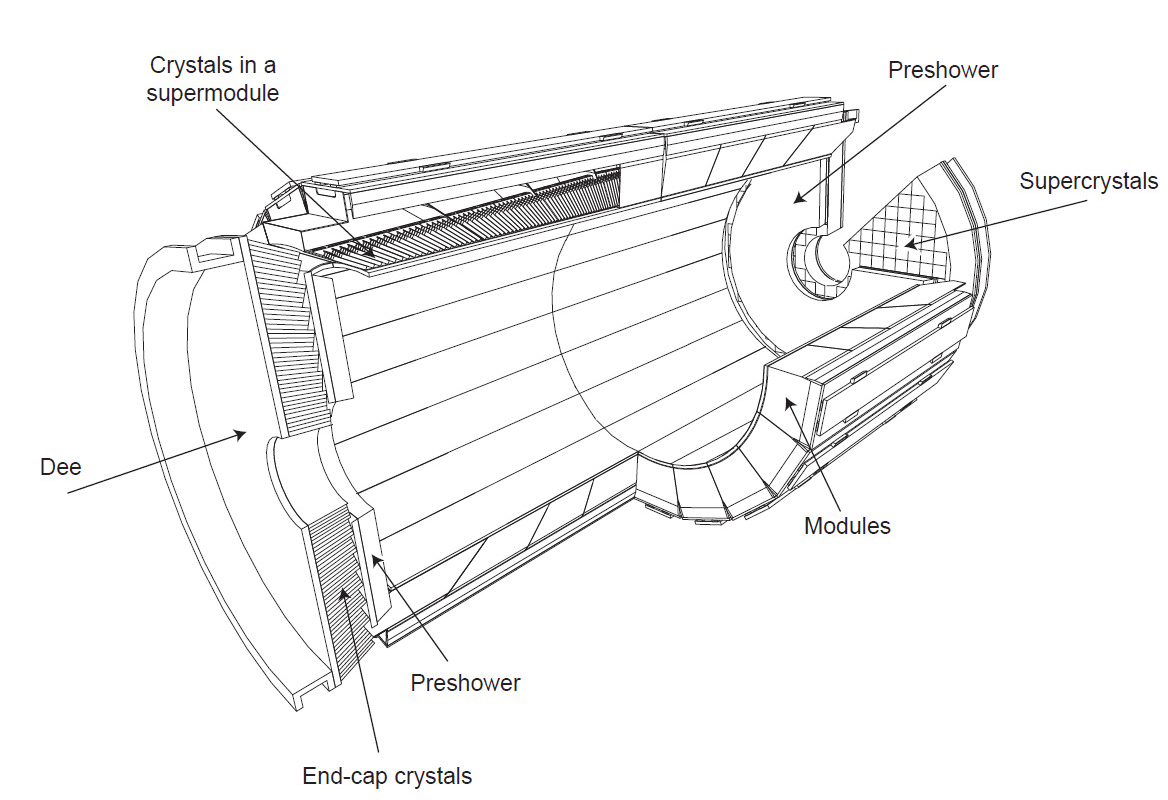
\includegraphics[width=\textwidth]{Figures/ECAL.png}
\caption{Geometric view of one quarter of the ECAL (top). Layout of the CMS electromagnetic calorimeter presenting the arrangement of crystal modules, supermodules, endcaps and the preshower in front (bottom) \cite{CMSexperiment}.}
\label{fig-ECAL}
\end{figure}

There are 75,848 within the ECAL, and are arranged into a barrel section (EB), covering a pseudorapidity range of $|\eta|<1.442$, and sealed by endcaps at each end of the cylindrical detector, thus extending the pseudorapidity range to $|\eta|<3.0$. The length of the crystals within the barrel are 230 mm and 220 mm in the endcap regions, which corresponds to $\sim26$ (EB) and $\sim25$ (EE) radiation lengths. The crystals are projective and also slightly off-pointing in position, $\sim3^\circ$ with respect to the IP. This configuration provides a full coverage and ensures that there are no cracks in the calorimetry that are aligned with particle trajectories. Within the barrel there is no longitudinal segmentation, and therefore the angle at which a photon is measured relies on the reconstructed PV from the silicon tracker. EB crystals are $2.2\times2.2$ cms$^2$ on the front face, and $2.86\times2.86$ cm$^2$ in the endcaps, giving rise to a total crystal volume of 11 m$^3$ and a weight of 92 t.

The barrel crystals are arranged into 36 supermodules (or superclusters), each containing 1,700 crystals, whereas the endcaps are arranged into two D-shaped segments comprising 3,662 crystals each. The final section of the ECAL is the pre-shower detector system (ES) placed directly in front of the endcaps at $1.65<|\eta|<2.6$ and can be visualised in Figure \ref{fig-ECALRapidity}. The ES is composed of 4,288 sensors, 137,216 silicon strip sensors, each $1.90\times61$ mm$^2$ with x-y view, and has a total of $\sim3$ radiation lengths. The purpose of the ES is provide improved separation of photons to $\pi^0$s.

\begin{figure}
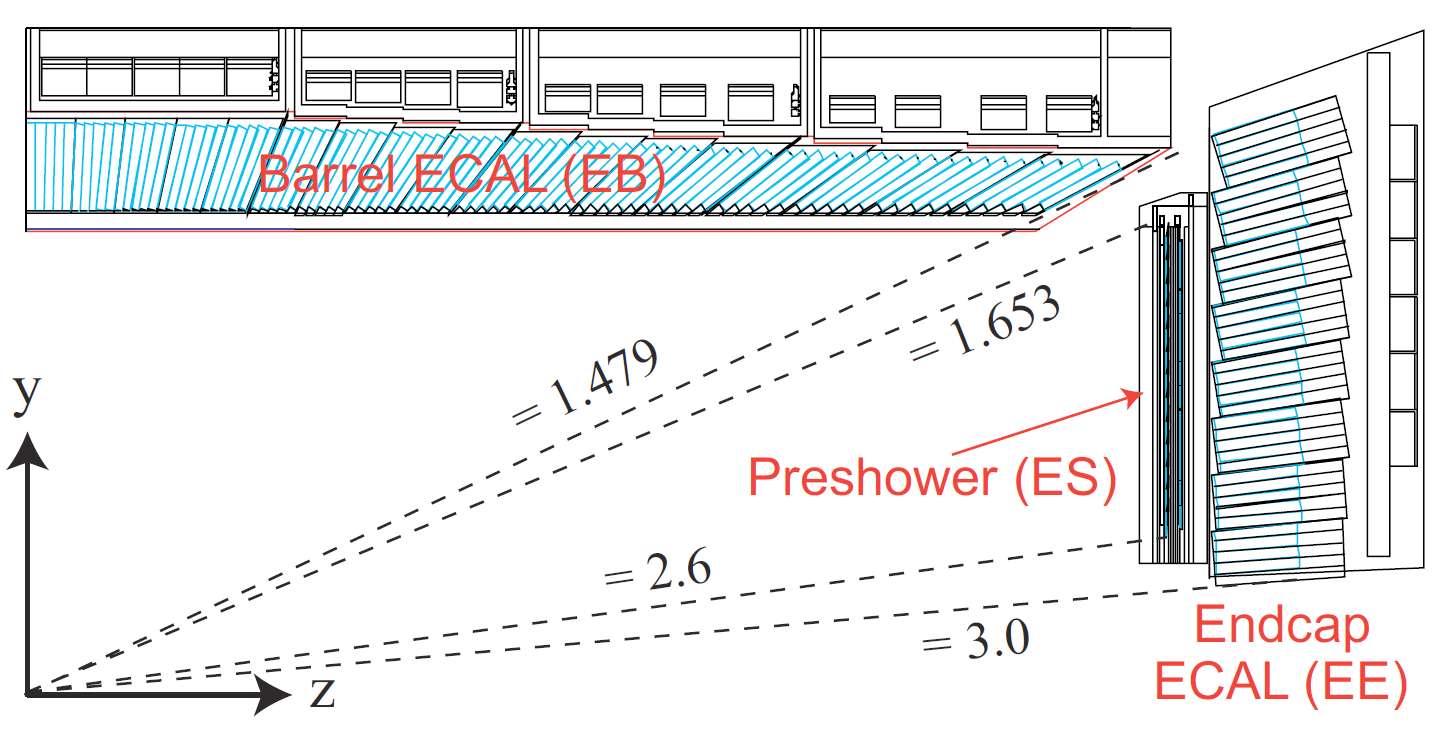
\includegraphics[width=\textwidth]{Figures/ECALRapidity.png}
\caption{Geometric view of one quarter of the ECAL (top). Layout of the CMS electromagnetic calorimeter presenting the arrangement of crystal modules, supermodules, endcaps and the preshower in front (bottom) \cite{CMSexperiment}.}
\label{fig-ECALRapidity}
\end{figure}

\subsection{Photodetectors} \label{subsec-Photodetectors}

The light read-out system for the barrel crystals comes in the form of Hamamatsu avalanche photodiodes (APD). There are two APDs for each crystal which are read in parallel, each measuring $5\times5$ mm$^2$ with a quantum efficiency (QE) of 75\%. The gain is set at $\sim50$ and they are insensitive to the 4 T magnetic field from the Superconducting Solenoid. The endcap crystals scintillation light is read out by vacuum photo-triodes (VPT), each with an area of 280 mm$^2$ with a 20\% QE and gain of $\sim10$. The barrel APDs are temperature sensitive ($\frac{1}{E}\frac{dE}{dT}\sim-2.3\%C^{-1}$) whereas the VPT sensitivity to temperature is assumed to be negligible relative to that of the crystals.  

\subsection{Performance of the ECAL throughout Run I} \label{subsec-ECALPerformance}

The energy resolution, $\frac{\sigma_E}{E}$ of the ECAL crystals can be parameterised by

\begin{equation} \label{eqn-ECALenergyresolution}
\left(\frac{\sigma_E}{E}\right)^2 = \left(\frac{A}{\sqrt{E}}\right)^2 + \left(\frac{B}{E}\right)^2 + C^2
\end{equation}

where A and B are the stochastic term for scintillation showers and noise term due to read-out electronics and photodetectors, respectively. C is a constant term which is a direct measure of the performance of the PbWO$_4$ crystals. We find that the performance of the ECAL can be attributed to inconsistencies in longitudinal light collection, noise due to the read-out electronics, and dead material within the detector causing energy leakages. The resolution was measured from test-beam data, using electrons within the energy rane of between 20 and 250 GeV. The values of A, B, and C have been measured to be 2.8\%, 12\%, and 0.3\%, respectively \cite{CMSexperiment}. The results were obtained in the absence of magnetic field, very little inert material in front of the calorimeter, and where the beam was aligned to the centres of the ECAL crystals. 

For unconverted photons within the energy range of interest for physics analysis ($\sim100$ GeV) we see that the energy resolution of the ECAL will be dominated by the constant term\footnote{For photons and electrons converting at small radii within the silicon tracker, the dominant contribution to the energy resolution arises due to radiation in the silicon tracker material combined with the effect from the magnetic field} in Equation \ref{eqn-ECALenergyresolution}. The result signifies that the performance of the ECAL is largely dependent on the quality of calibration and monitoring during data-taking periods. 

\begin{figure} 
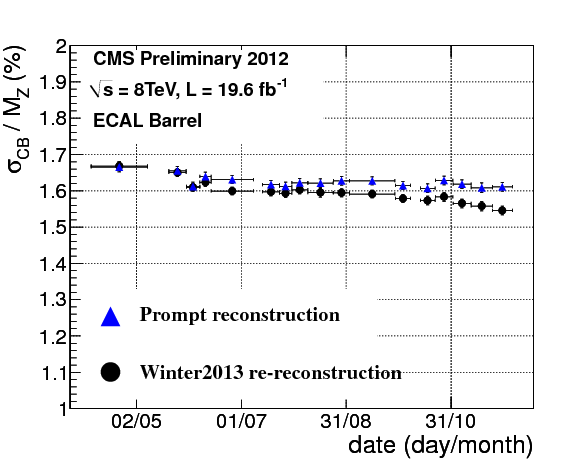
\includegraphics[width=0.50\textwidth]{Figures/EcalInvariantMass.png}
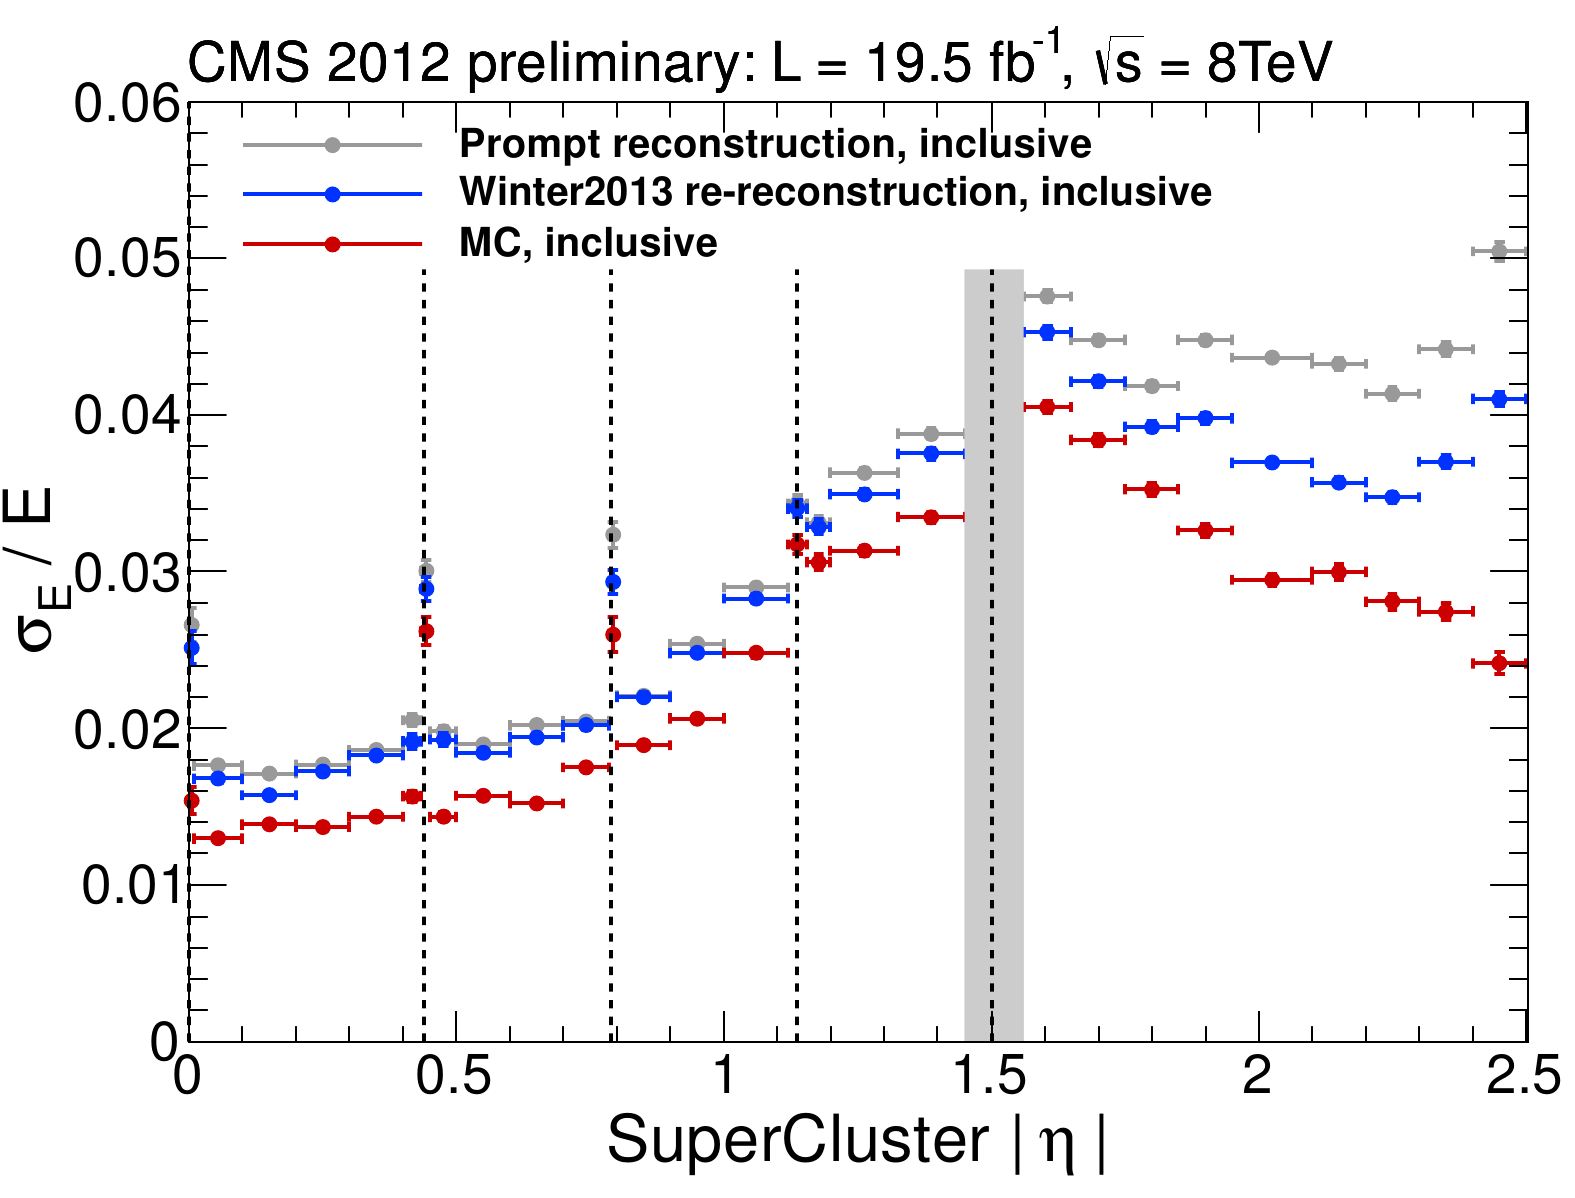
\includegraphics[width=0.52\textwidth]{Figures/EcalEtaInclusive.png}
\caption{Left: The mass resolution of the Z peak, reconstructed from its di-electron decay mode, as a function of time for the barrel. Right: Relative electron (ECAL) energy resolution unfolded in bins of pseudo-rapidity $\eta$ for the barrel. \cite{ECALPerformance}.}
\label{fig-ECALperformance}
\end{figure}


Figure \ref{fig-ECALperformance} shows the invariant mass resolution as a function of time for prompt and re-reconstructed electrons (left), and the relative electron resolution as a function of pseudorapidity, $\eta$, (right) both used a $Z \to e^+e^-$ sample. 

The electron energy resolution, $\sigma_e/E$, is derived from the peak width of $Z \to e^+e^-$ decays and fitting in bins of $\eta$ using an unbinned maximum likelihood fit to the invariant mass distribution of $e^+e^-$ pairs. We find that the energy resolution is greater than 2\% in the eta range $|\eta| < 0.8$, and ranges from 2 - 5\% in other regions. We can also see the effect created by the excess of material upstream of the ECAL in the regions where $|\eta| > 1$, also near the detector cracks (shown as a grey line) between ECAL modules. The difference between data (blue) and MC (red) is thought to arise due to flaws in simulation, such as a mismodelling of the upstream material.

%\cite{CMS-DP-2013-007}

\section{Hadron Calorimeter} \label{sec-HadronCalorimeter}

\subsection{Overview}

The Hadron Calorimeter (HCAL), shown in Figure \ref{fig-HCAL}, lies directly after the ECAL within the volume of the superconducting solenoid, and is designed to measure energy deposits from hadron showers and clusters of collinear high-energy hadronic particles known as jets. A key role of the HCAL is to measure the missing transverse energy (MET) produced by events containing neutrinos, and possible events that could be associated with new physics that may be seen at higher energies. In order to produce such a precision measurement, the HCAL must have an extremely high jet energy resolution and be completely hermetic in $\phi$. 

The HCAL is a sampling calorimeter, composed of alternating layers of absorbing large brass plates and plastic scintillation tiles. Because the precision of the energy measurement depends on the total amount of the hadronic shower detected, the material must be thick enough to absorb the majority of the event. The size restriction for the HCAL is limited to the distance between the end of the ECAL ($r=1.77$ m) to the inner superconducting solenoid ($r=2.95$ m). In order to efficiently measure the full shower, and therefore energy deposit, an outer section of the HCAL (HO) has been placed just after the solenoid and between the muon system which can then also be used as an extra layer of absorbing material with a thickness of 11.4 interaction lengths ($\lambda_l$). There are four segments of the HCAL in total: the HCAL barrel (HB), endcaps (HE), outer HCAL (HO), and forward calorimeter (HF). The barrel and endcaps combined covers an area with pseudorapidity up to $|\eta|<3.0$, and the forward segment covers the region up to $|\eta|<5.0$.  

\begin{figure} 
\begin{center}
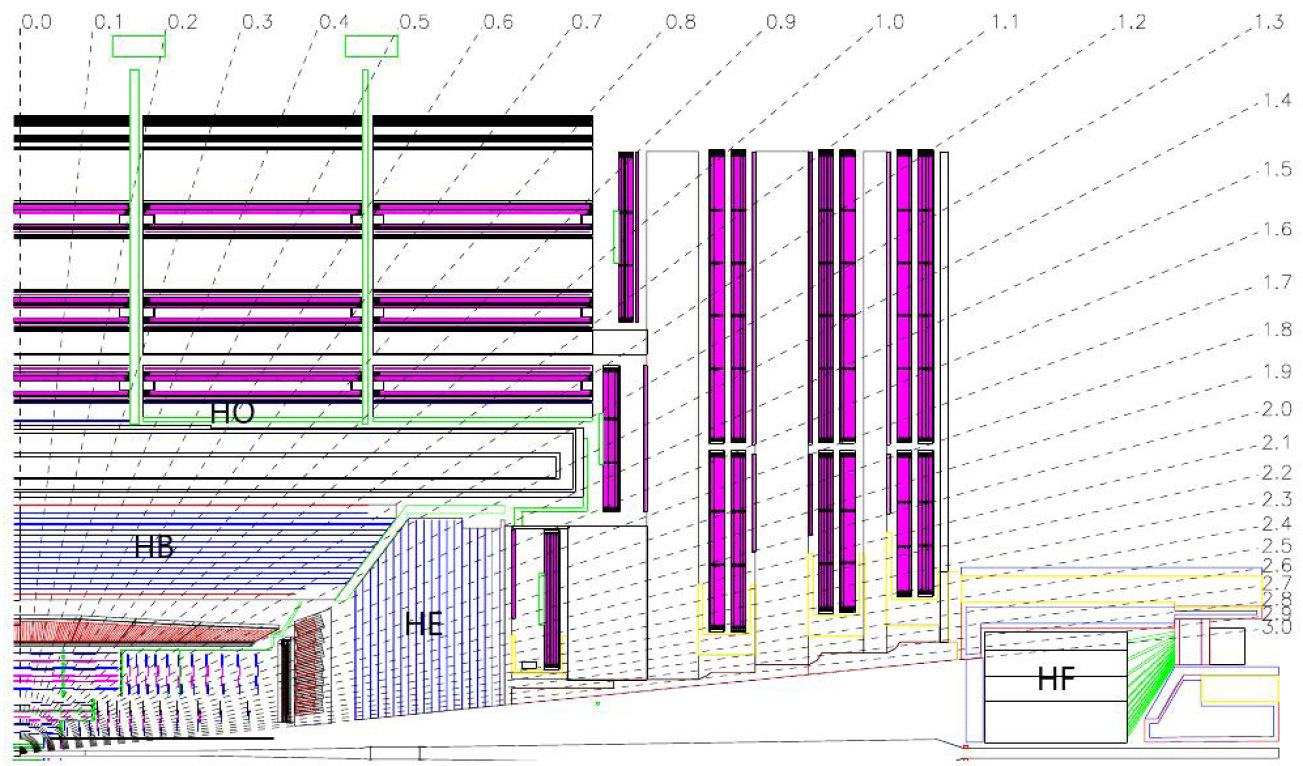
\includegraphics[scale=0.3]{Figures/HCAL.png}
\end{center}
\caption{Longitudinal view of one quarter of the detector in the $r-\eta$ - plane, showing the positions of the HCAL parts: hadron barrel (HB), hadron outer (HO), hadron endcap (HE) and hadron forward (HF) \cite{CMSexperiment}.}
\label{fig-HCAL}
\end{figure}

\begin{table} 
\begin{center}
\begin{tabular}{lccccc}
\hline
\hline
 & \textbf{HB/HO} & \textbf{HE $|\eta| \leq 2.5$} & \textbf{HE $|\eta|>2.5$} & \textbf{HF $|\eta| \leq 2.5$} & \textbf{HF $|\eta|>2.5$} \\
\hline
\textbf{$\Delta \eta \times \Delta \phi$} & $0.087 \times 0.087$ & $0.087 \times 0.087$ & $0.175 \times 0.175$ & $0.175 \times 0.175s$ & $0.175 \times 0.35$ \\
\hline
\hline
\end{tabular}
\end{center}
\caption{Tower segmentation in azimuthal and polar angle for the hadronic barrel, endcap and forward calorimeter \cite{HCALTdr}.}
\label{tab-HCALGranularity}
\end{table}

There are approximately 90,000 scintillators installed within the HB and HE combined. Light that is collected by the plastic scintillating tiles is read about by wavelength-shifting fibres (WSF) that are embedded within the units, which are then transported through transparent fibres to hybrid photo-detectors (HPD) encompassing 19 independent pixels. Each scintillator has a granularity of $\Delta \eta \times \Delta \phi = 0.087 \times 0.087$ for $|\eta|<1.6$ and $\Delta \eta \times \Delta \phi = 0.17 \times 0.17$ for $|\eta| \ge 1.6$, whereas the forward segment changes with respect to pseudorapidity as $\Delta \eta \times \Delta \phi = 0.175 \times 0.175$ at $|\eta| = 3.0$ to $\Delta \eta \times \Delta \phi = 0.175 \times 0.35$ at $|\eta| = 5.0$ \cite{HCALTdr}, as seen in Table \ref{tab-HCALGranularity}. The forward section of the HCAL is placed 11.2 m from the IP in order to reconstruct particles boosted in the forward direction, and is expected to experience a much higher flux of particles at higher energy (760 GeV) than the rest of the HCAL (100 GeV) at $\sqrt{s}=14$ TeV \cite{HCALUpgradeTdr}. It is composed of 5 mm thick steel absorber plates, each with quartz fibres implemented as an active medium. The quartz fibres detect \v{C}erenkov light produced from the electromagnetic component of particle showers.

\subsection{Performance of the HCAL in Run I}   



\section{Superconducting Solenoid} \label{sec-SuperconductingSolenoid}

The CMS Superconducting Solenoid, shown in Figure \ref{fig-SuperconductingSolenoid}, is the most powerful hadronic magnet in the world, 100,000 times stronger than the Earth's magnetic field and stores enough energy to melt 16 tonnes of gold, and the most essential feature of the detector. In order to achieve a good momentum resolution in such a detector, without making tight cuts on muon chamber resolution and alignment, a powerful magnetic field was chosen. A large bending power can be achieved by a modestly sized solenoid, as long as it is a high-field superconducting one, due to the bending beginning at the primary vertex. The requirement for the bending power of the solenoid is dictated by the narrow states decaying into muons, and by the unambiguous determination of the sign for muons with a momentum of around 1 TeV/c. In order to obtain a precision measurement, a momentum resolution of $\Delta p/p\approx10\%$ at p = 1 TeV/c. A suitable length to radius ratio is required to obtain a good momentum resolution in the forward region.  

\begin{table} 
\begin{center}
\begin{tabular}{|l|c|}
\hline
	\multicolumn{2}{|c|}{\textbf{Superconducting Solenoid Parameters}} \\
\hline
	\textbf{Parameter} & \textbf{Value} \\
\hline
	Field (T) & 4 \\
	Length (m) & 12.9 \\
	Weight (t) & 250 \\
	Inner bore (m) & 5.9 \\
	Current (kA) & 19.5 \\
	Number of turns & 2168 \\
	Stored energy (GJ) & 2.7 \\
	Hoop stress (atm) & 64 \\
\hline
\end{tabular}	
\end{center}
\caption{Parameters of the LHC superconducting solenoid \cite{MagneticField}.}
\label{tab-SolenoidParameters}
\end{table}

Approaching 13 m in length, and 6 m in diameter, the solid mass weights approximately 250 t at an operating temperature of $-268.5^\circ C$ -- a degree warmer than outer space. Originally designed to run with a uniform magnetic field of 4 T within the 5.9 m bore, the eventual operating level was set to 3.8 T in order to increase the lifetime. Such a magnetic field requires a return yoke, which can be viewed in the CMS schematic in Figure \ref{fig-CMSDetector}, of which the return field is large enough to saturate 1.5 m of iron and weighs 12,500 t. This allows four muon stations to be integrated within the return yoke, ensuring robustness and full geometric coverage. The magnet and return yoke use almost twice as much iron as the Eiffel Tower. The solenoid is composed of four layers of high-purity niobium-titanium cable coextruded with a aluminium-stabilised conductor as used in previous experiments, such as ALEPH and DELPHI at LEP, and H1 at HERA. However, the huge increase in certain parameters, such as magnetic field strength, ampere turns, and stored energy, which can be seen in the parameters listed in Table \ref{tab-SolenoidParameters} \cite{PTDR2}. 

\begin{figure} 
\begin{center}
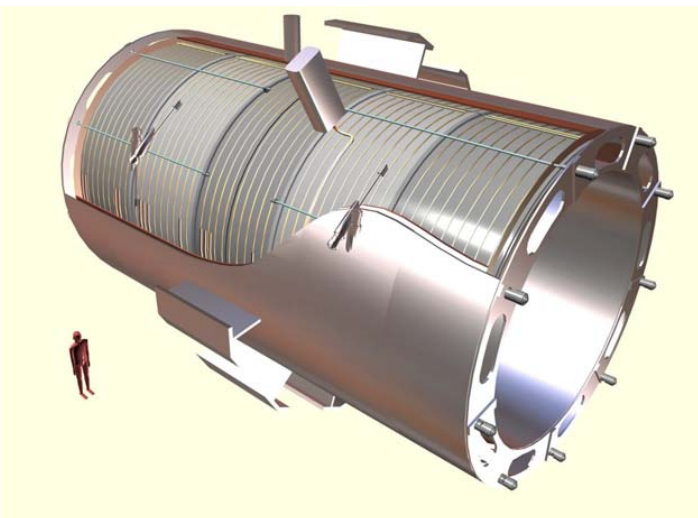
\includegraphics[scale=0.5]{Figures/SuperconductingSolenoid.png}
\end{center}
\caption{ General artistic view of the 5 modules composing the cold mass inside the cryostat, with details of the supporting system (vertical, radial and longitudinal tie rods) \cite{CMSexperiment}.}
\label{fig-SuperconductingSolenoid}
\end{figure}


\section{Muon System} \label{sec-MuonSystem}

The final sub-detector, or rather set of sub-detectors, lying between each wheel of the iron return yoke, is the muon system (Figure \ref{figCMSLongitudinalView}). The muon system plays a huge role in detecting signatures of interest, such as processes with extremely large backgrounds, and which are expected to increase in Run II. Signatures such as a the so called ``gold-plated" decay of a standard model Higgs decaying to two Z bosons, both of which decay into two muons ($H \to ZZ \to \mu^+ \mu^- \mu^+ \mu^-$), are ideal candidates because the best mass resolution can be achieved as muons are much less effected than electrons by radiative losses within the tracker material. Due to the relative ease of detecting muons, this decay channel (discovered in Run I, \cite{}) highlights the discovery potential for muon final state decay modes and the demand for such a wide angular coverage within the muon detection system. 

Precise and efficient muon measurements were a central theme in the design of the CMS experiment, as can be seen from the name. There are three functions which the muon system serves: identification of muons, momentum measurements, and triggering. All of these functions are made  possible when used in conjunction with the superconducting solenoid and its flux return yoke. The system was designed to measure the charge and momentum of muons over the full kinetic range of the LHC. The design of the muon system was based around the nature of the solenoid magnet, thus it is composed of a cylindrical barrel section surrounded by two planar endcaps to provide fully hermetic coverage. The design of the system had corresponds to 25,000 m$^2$ of detection planes and thus the muon chambers must be robust, reliable, and also inexpensive. Therefore, three types of gaseous particle detectors were implemented: drift tubes (DT), cathode strip chambers (CSC), and resistive plate chambers (RPC). 

\begin{figure}
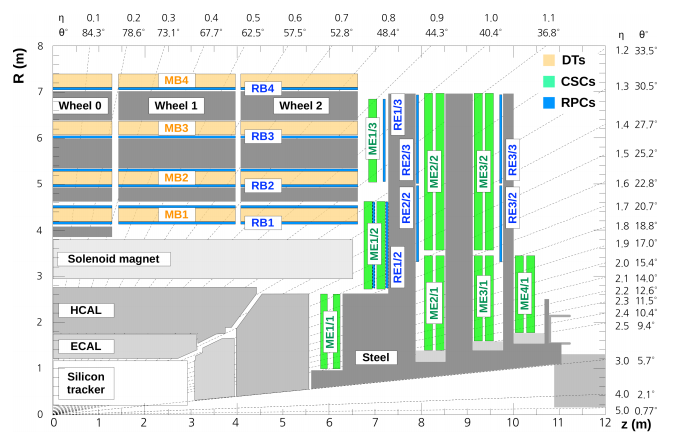
\includegraphics[width=\textwidth]{Figures/CMSLongitudinalView.png}
\caption{Layout of one quadrant of CMS. The figure shows the four DT stations in the barrel (MB1-MB4, yellow), the four CSC stations in the endcap (ME1-ME4, green), and the RPC stations (RB1-RB4 and RE1-RE3) \cite{CMSexperiment}.}
\label{fig-CMSLongitudinalView}
\end{figure}

Drift tubes with standard rectangular drift cells are implemented in the muon barrel section where the neutron-induced background is small, the muon rate is low, and the 4 T magnetic field is uniform and mostly contained within the steel return yoke. Covering a pseudorapidity region of $|\eta|<1.2$, the barrel drift tube chambers are arranged into four layers integrated within the return yoke. The first three layers contain 8 chambers which measure the muon coordinates in the $r-\phi$ bending plane, and 4 that measure $z$ along the beam-line. The fourth station is the same except that it does not measure $z$. The arrangement and number of chambers in each station were chosen to provide efficient rejection of background hits and linking muon hits from different stations into one single track.

In contrast to the barrel region, the background and muon rates are high and the magnetic field is non-uniform. For this region cathode strip chambers are used. The CSCs have an extremely fast response time, resistance to radiation, fine segmentation, and can identify muons within a pseudorapidity range of $0.9 < |\eta| < 2.4$. Again there are four layers of chambers interspersed between the return yoke plates, however they are perpendicular to the beam. The strips are positioned radially outward and provide precise measurements in the $r-\phi$ bending plane. Each CSC comprises 6 layers, providing robust pattern recognition and rejection of backgrounds, efficiently matching hits in the CSCs to those in the tracker.

The third sub-detector in the muon system is implemented to serve as a complimentary, dedicated trigger system composed of resistive plate chambers (RPC) in both the barrel and endcaps. The decision to include the RPCs was based on the uncertainty in the eventual background rates and ability to measure the correct beam-crossing time when the LHC reaches design luminosity. The RPCs are able to operate in high rate environments by using fast, highly-segmented, and independent trigger, but provide a more accurate position resolution than the DTs or CSCs. The p$_T$ threshold is sharp over a large segment of the pseudorapidity range, $|\eta|<1.6$. 

\subsection{Performance of the muon system in Run I} \label{subsec-MuonSystemPerformance}

During the Run I data taking period, CMS muon reconstruction was performed using the silicon inner tracker in coincidence with up to four of the available gas-ionisation muon chambers: DTs, CSCs, and RPCs. Standard CMS muon tracks can be reconstructed independently both in the inner tracker and in the muon system, where tracks are labelled tracker and standalone-muon tracks, respectvely. When reconstructing a global muon, we rely on local reconstruction of objects within each individual muon chamber. Each muon chamber uses different techniques in reconstructing charged particles that cross the chambers, however every case relies on the ionisation of gas within the volume of the detector.  

Basic objects that traverse the gas within the chambers are ionised, read out, and reconstructed as hits. Hits are defined as spatial points with assigned uncertainties and segments, which are obtained by fitting straight lines to the reconstructed hits \cite{Chatrchyan:2013sba}. For the reconstruction of standalone-muon tracks, a matching tracker track is pinpointed by comparing the parameters of each and propagating onto a common surface --- which is known as the outside-in method. Global muons are fitted by combining hits from each of the tracker and standalone-muon tracks and using the Kalman-filter technique. 

RPC muons are reconstructed in a similar fashion to tracker muons by requiring only two reconstructed hits in different layers of the RPC chambers. The matching criteria for each of these types of reconstructed hits is the distance and pull between their positions in a local x and y frame, where we define the pull as the residual between the extrapolated positions over the combined uncertainty \cite{MUO-12-482}. The pulls and residuals for track segment matching has been studied previously \cite{Chatrchyan:2013sba}. By reconstructed tracker muons in this manner we drastically reduce the probability of reconstructing punch-through hadrons. By combining different algorithms we are able to increase the efficiency of correctly reconstructing a muon.

The efficiency of correctly reconstructing a muon track is studied by way of the tag-and-probe method (see Section \ref{subsec-LeptonEfficiencies}) using a sample of Z bosons decaying to muons. The analysis is conducted in a semi-Tight muon selection regime, whereby the candidate is required to be identified as a RPC muon with hits matched in at least three RPC layers, and two matched hits in two muon stations. Thr semi-Tight muon selection does not include particle flow (PF), see Section \ref{subsec-PFAlgorithm}, identification and isolation cuts. The results yield and increase of around 3\% in the efficiency compared to previous measurements \cite{MUO-12-482}, and can be seen in Figure \ref{fig-MuonEfficiencies}. The efficiency lies above 99\% in for most p$_T$ and $\eta$ regions. 

\begin{figure} 
\begin{center}
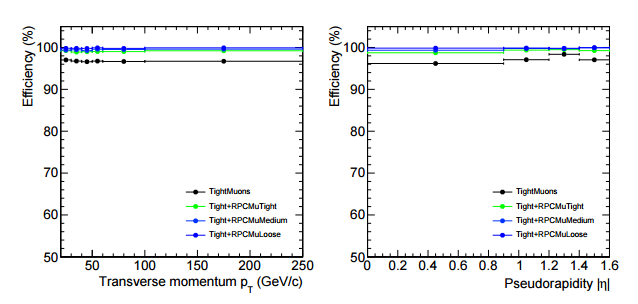
\includegraphics[width=\textwidth]{Figures/MuonEfficiencies.png}
\end{center}
\caption{RPCMuon efficiencies on top of the semi-Tight muon selection in p$_T$ and $|\eta|$. \cite{MUO-12-482}}
\label{fig-MuonEfficiencies}
\end{figure}


\section{Trigger and Data Acquisition} \label{sec-Trigger}

At the LHC design energy of $\sqrt{s}=14$ TeV, the proton-proton collision frequency reaches up to 40 MHz when operating with 25 ns bunch spacing. Depending on the luminosity, a number of collisions will occur at each crossing of the protons, but since every event produces $\sim1$ MB of raw data, this corresponds to a total of $\sim 40$ TB s$^{-1}$. Also, at the design luminosity of $\mathcal{L} = 10^{34}$ cm$^{-2}$ $s^{-1}$, around 20 inelastic events will be superimposed onto events of interest, known as pile-up (PU). The amount of resulting data is much too large to store and process, and thus a filtering system for interesting events is implemented to reduce the total number of events recorded. This is the trigger system, and begins the process of event selection in the CMS experiment. The rate reduction capability is designed to be at least a factor of $10^6$ for the combination of L1 Trigger and HLT.

The trigger is designed as a two-stage system: Level 1 (L1) Trigger, and High-Level Trigger (HLT), respectively. The L1 trigger is a hardware system consisting mostly of custom-designed, highly programmable electronics, located partly on the detector and partly in the underground control room approximately 90 m from the detector itself. The L1 trigger makes a decision based on information from only the muon system and calorimetry, and is shown in Figure \ref{fig-L1Trigger}. The tracker information is not used in making trigger decisions due to the length of time needed to reconstruct tracks exceeding that of the L1 trigger. The data used is coarsely segmented, with the high resolution data being held in pipeline memories in the front-end electronics. Constructed with a design output rate limit of 100 kHz, this in actuality translates in practice to a maximal output rate of $\sim30$ kHz when taking into account a safety factor of 3. We can divide the L1 trigger into different components: local, regional, and global components. The first components are the Local Triggers, also named Trigger Primitive Generators (TPG), and are collections of information from deposits in calorimeter trigger towers and track segments, or hit patterns in the muon chambers, respectively. Next are the Regional Triggers that combine the information obtained and use pattern logic in order to determine the rank and sort of trigger object, such as an electron or muon candidates. The rank can then be defined as a function of energy or momentum and quality of the deposit, reflecting the confidence level assigned to the L1 parameter measurements. The final components are the Global Calorimeter and Global Muon Triggers, assigning the highest rank calorimeter and muon objects throughout the detector. The candidates are then transferred to the Global Trigger, the highest component of the Level 1 hierarchy, which then makes a decision of whether to accept or reject the event for evaluation by the HLT. 


\begin{figure} 
\begin{center}
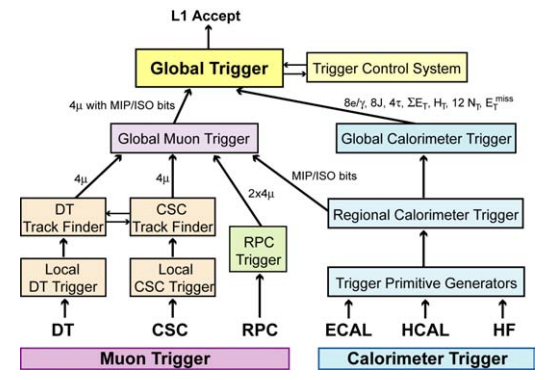
\includegraphics[scale=0.5]{Figures/L1Trigger.png}
\end{center}
\caption{Architecture of the Level 1 trigger \cite{CMSexperiment}.}
\label{fig-L1Trigger}
\end{figure}

The HLT is a software system residing in a CPU filter farm containing around 1000 commercial processors. The advantage of the HLT is that it has access to the full event information from the entire detector simultaneously, including event information unavailable on the timescale of the L1. It can then perform complex calculations, similar to that performed in the analysis off-line software, by constantly evolving complex algorithms, resulting in a highly flexible trigger system. The event rate at the HLT level is reduced to $\sim300$ Hz and a final data rate of $300$ MBs$^{-1}$ recorded on a large storage disk (the Storage Manager) at the experimental site. The data is later transferred to the base tier (Tier 0) of The Grid computing network for further processing and then physics analysis.

\subsection{Performance of the Trigger in Run 1} \label{subsec-TriggerPerformance}

The majority of physics analyses in CMS that published findings using Run I data at a centre-of-mass of $\sqrt{s}=8$ TeV used complicated triggers, where multiple categories of objects may be incorporated, such as jets and leptons. This category of trigger looks at the whole event topology and calculates such quantities as the total scalar energy, H$_T$, or missing transverse energy. 

At the new unprecedented energies recorded by the LHC, gluon fusion is the most dominant process in proton-proton collisions, and as a result the rate of production for top-quark pairs increases and the LHC essentially becomes a top factory. As a result, the production cross-section for top pairs is one of the most fundamental measurements to compute. The measurement is computed using the semi-leptonic channel, such that one of the top quarks will decay to a b-jet and a lepton (electron or muon) and a neutrino, and the other will decay to a b-quark and two jets \cite{Chatrchyan:2012ria, SemiLeptPAS}. 

In order to accommodate the high instantaneous luminosity and pile-up throughout Run I, various triggers were used: Lepton triggers with very tight identification and calorimeter isolation requirements, jets and PF jets were limited to the central region. Similar techniques were implemented at the L1 stage of reconstruction. Muons were defined within the central region ($|\eta| < 2.1$), charged hadron subtraction was introduced to deal with pile-up mitigation, and during the second half of the 2012 running period online jet energy calibrations were implemented which resulted in higher E$_T$ thresholds in three-jet trigger paths. 

The lepton plus jets efficiency is measured as the product of two independent efficiency measurements, $\epsilon_{Lep.} \times \epsilon_{Had.}$ using the tag-and-probe method with simulated Drell-Yan and $t\bar{t}$ samples, as described in Section \ref{subsec-LeptonEfficiencies}. To estimate the top acceptance simulated events were used and are corrected for the trigger efficiency measured in data. 

Figure \ref{fig-SemiLeptEfficiencies} shows the turn-on curve for the efficiency for selecting the hadronic leg (p$_T$ of the 4th jet) of the electron plus jets channel, and the dependency of the efficiency on the number of reconstructed primary vertices. The offline selection of the p$_T$ for the jets was designed to assure a plateau behaviour of the scale factors, such that there is no variation with respect to MC sample or jet energy calibrations. From the variation of the scale factors, a systematic uncertainty of 2\% (1.5\%) for the electron (muon) scale factors cover the variation around their value of 0.995 (0.987) \cite{CMSTriggerPerformance}. 

\begin{figure} 
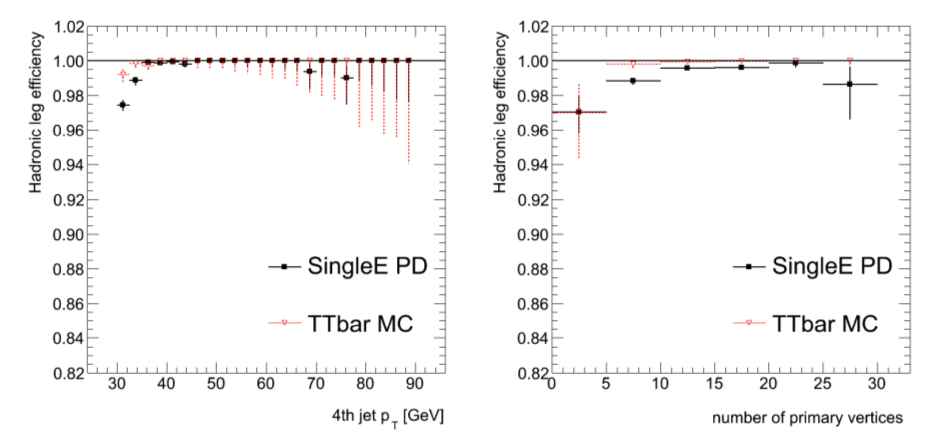
\includegraphics[width=\textwidth]{Figures/SemiLeptTriggerEfficiencies.png}
\caption{Top Triggers: Efficiency of the hadronic leg for the electron plus jets paths in 2012 versus the p$_T$ of the 4th jet (left) and the dependence with respect to the number of vertices (right). \cite{CMSTriggerPerformance}}
\label{fig-SemiLeptEfficiencies}
\end{figure}
